
\graphicspath{{chapters/paper1/figures/}}


\chapter{Paper 1}
{\Huge \textbf{High Resolution Data Assimilation of Cardiac
  Mechanics}}

% \pagebreak
% \clearpage
\newpage
\renewcommand{\thefootnote}{\fnsymbol{footnote}}

\section*{High Resolution Data Assimilation of Cardiac Mechanics}


% \begin{center}
Gabriel Balaban$^{1,2,5}$\footnotemark[\value{footnote}],
Henrik Finsberg$^{1,2,5}$\footnotemark,
Hans Henrik Odland$^{4,5,7}$,
M. E. Rognes$^{1,3}$,
Stian Ross$^{4,5}$,
Joakim Sundnes$^{1,2,5}$, and
Samuel Wall$^{1,5,6}$


\footnotesize
\begin{enumerate}[itemsep=-2mm]
\item{Simula Research Laboratory, Lysaker, Norway}
\item{Department of Informatics, University of Oslo, Oslo, Norway}
\item{Department of Mathematics, University of Oslo, Oslo, Norway}
\item{Faculty of Medicine, University of Oslo, Oslo, Norway}
\item{Center for Cardiological Innovation, Oslo, Norway}
\item{Department of Mathematical Science and Technology, NMBU, \r{A}s,
    Norway}
\item{Department of Pediatrics, Oslo University Hospital, Oslo, Norway}
\end{enumerate}
\normalsize

\subsection*{Abstract}


% \clearpage
% \begin{abstract}

Computational models of cardiac mechanics, personalized to a patient, offer access 
to mechanical information above and beyond direct medical imaging.
Additionally, such models
can be used to optimize and plan therapies in-silico, thereby reducing risks and
improving patient outcome. Model personalization has traditionally been achieved by data
assimilation, which is the tuning or optimization of model parameters
to match patient observations.
Current data assimilation procedures for cardiac mechanics are limited in their ability
to efficiently handle high dimensional parameters.
This restricts parameter spatial resolution, and thereby the ability
of a personalized model to account for heterogeneities that are often present in
a diseased or injured heart.
In this paper we address this limitation by
proposing an adjoint-gradient based data assimilation method
that can efficiently handle high-dimensional
parameters. We test this procedure on a synthetic data set,
and provide a clinical example with
a dyssynchronous left ventricle with highly irregular motion.
Our results show that the method efficiently handles a high dimensional
optimization parameter, and produces an excellent agreement
for personalized models to both synthetic and clinical data.

% \end{abstract}
\footnotetext{Both of these authors contributed equally to this work.}
% \maketitle

% \clearpage
\newpage
\section{Introduction}
Computational models of cardiac mechanics, personalized to the level of the individual 
through the use of clinical imaging, have potential to be a powerful aid in the diagnosis and 
treatment of cardiac disease.  By relating image-based data to fundamental physical 
processes, models can give additional insight into the function or dysfunction of the 
individual's heart, beyond what can be directly measured or observed in the images. 
This is becoming more important as the resolution and accuracy of clinical imaging continues to 
improve.  This increasingly detailed data combined with biophysical models has promise 
in analysis of regionally and temporally resolved differences in the mechanics of the heart, 
important in diseases such as heart failure and the application of cardiac resynchronization therapy. 

A key step in making these clinically useful cardiac mechanics models is proper data assimilation from patient observations into a fit model. This involves the optimization, or tuning, of individual model parameters in order to make the model match the observations of the patient's heart.  Over the last decade several data assimilation methods have been developed and proposed for this problem. The earliest studies employed gradient based optimization in order to minimize the discrepancy between model-derived data and clinical observations.  The gradients necessary for these optimizations were calculated using direct differentiation \cite{sermesant2006cardiac}
or finite difference \cite{augenstein2005method, gao2015parameter, Wang2009}.
More recent efforts include the use of global optimization methods:
in particular genetic algorithms \cite{mojsejenko2014estimating,
sun2009computationally}, a Monte Carlo method \cite{neumann2014robust},
subplex algorithm \cite{wong2015velocity}, and parameter sweeps \cite{asner2015estimation, hadjicharalambous2015analysis}.
Finally, reduced order unscented Kalman filtering has also been successfully applied as
a data assimilation tool for patient-specific model creation \cite{chabiniok2012estimation,
xi2011myocardial, Marchesseau2013}.

The increasingly large amount of easily obtainable geometric and motion data, 
however, is a challenge for data assimilation into personalized computational models 
using the techniques mentioned above.  This is as the computational 
expense scales badly with the number of model parameters to be fit. In the 
case of the Kalman filtering strategies, at least one extra evaluation 
of the model is required per additional model parameter to be optimized.
The calculation of model-data mismatch gradients by finite difference 
or direct differentiation suffers from the same limitation. Global methods 
on the other hand are affected by the curse of dimensionality; that is, 
a rapid expansion of the space of parameters that must be searched as the number 
of dimensions increases. For high dimensional problems 
the run-time needed to carry out a global search can be computationally prohibitive.

In contrast, the calculation of a functional gradient by the adjoint formula is 
nearly independent of the number of optimization parameters, requiring one forward and one backward 
adjoint solve of the mathematical model. The forward solve is typically needed to evaluate the functional, 
and the evaluation of the gradient at the same point requires only an additional backward solve of the adjoint system.
Furthermore, this backward solve is always linear, 
and therefore computationally less expensive than the forward solve 
if the mathematical model is nonlinear. These methods have been widely explored in model optimization, 
with adjoint-based data assimilation techniques having previously been
employed for cardiac mechanics, specifically using linear elastic models and
clinical data~\cite{Delingette2012, sundar2009biomechanically}, and
also nonlinears model combined with experimental
data~\cite{balaban2016adjoint}.

In this work we provide an improved data assimilation pipeline for high resolution optimization,
demonstrating the parameterization of mechanical contraction in high spatial resolution 
driven by 4D echocardiography patient data. This high dimensional optimization problem 
is efficiently solved using an adjoint gradient based technique, described in detail 
in our previous work \cite{balaban2016adjoint}. We demonstrate our method on the pathological 
case of a dyssynchronous left ventricle, which has complex and irregular motion, 
as well as on a synthetic case consisting of data generated by our mechanical model. 
This study is to the best of our knowledge the first to use adjoint-based data assimilation 
for nonlinear cardiac mechanics with clinical data, and the first to consider the 
resolution of a parameter at the same scale as the discretization of the cardiac geometry.
These are important considerations as better understanding of myocardial properties 
emerges and the collection of high resolution clinical data continues to expand.

The rest of this paper is organized as follows: In
Section~\ref{paper1:sec:methods} we present a mathematical model that
accounts for the three main drivers of ventricular mechanics; blood
pressure, tissue elasticity and muscle contraction.  
We also describe clinical measurements of a patient suffering from dyssynchrony, and our data assimilation procedure
for fitting the model to these measurements.
Numerical results are presented in Section~\ref{paper1:sec:num_results}, and discussed in
Section~\ref{paper1:sec:discussion}. Finally, we provide some concluding
remarks in Section~\ref{paper1:sec:conclusion}.


\section{Materials and Methods}
\label{paper1:sec:methods}

\subsection{Wall motion modelling}

\label{paper1:sec:wall_motion}
In order to estimate the position of the myocardial walls through
the cardiac cycle we adopt a continuum mechanics description of
cardiac wall motion. In this description we consider a fixed left
ventricular reference geometry $\Omega$, with endocardial boundary
$\lvendo$, and basal boundary $\basebound$.

Our fundamental quantity of interest is the vector valued displacement
map $\uvec(\mathbf{X})$, where $\mathbf{X} \in \Omega$.  At any given
point in time in the cardiac cycle, $\uvec(\mathbf{X})$ relates
the current geometry $\omega$ to the reference geometry by
 \begin{equation}
{\bf X} + {\bf u}({\bf X}) = {\bf x}, \quad {\bf x} \in \omega, \quad {\bf X} \in \Omega. 
\end{equation}

Assuming that the cardiac walls are in equilibrium,
it is possible to determine the value of $\uvec$ from the principle of
virtual work
\begin{equation}
  \label{paper1:eq:work-balance}
  \delta W(\uvec) = 0,
\end{equation}
which states that the virtual work, $\delta W(\uvec)$, of all forces
applied to a mechanical system vanishes in equilibrium. For our ventricular wall motion
model, the virtual work $\delta W(\uvec)$, is given by
\begin{equation}
\begin{aligned}
\label{paper1:eq:workdef}
 \delta W(\uvec, p) &= \int_{\Omega} \FPK : \Grad \ \du \ dV 
		  + \int_{\Omega} (J - 1) \dpre + p J \F^{-T} : \Grad \ \du \ dV  \\
		 &+ \plv \int_{\lvendo} J \F^{-T} \Nvec \cdotp \du \ dS 
		  +  \int_{\lvbase}  k \uvec \cdotp \du \ dS.
 \end{aligned}
\end{equation}
Here we have introduced the hydrostatic pressure $p$ in order to enforce the 
incompressibility constraint $J =1$, with $J = \det \F = \det  \left(\Grad \ \uvec + \mathbf{I}\right)$, 
and $\mathbf{I}$ being the second order identity tensor. 
Furthermore, $\Nvec$ denotes the unit outward normal vector, $k$ 
the constant of a spring that we introduce at the basal boundary, and $\plv$ the intra-ventricular 
blood pressure. The virtual variables $\du$ and $\dpre$ are test functions whose values
are arbitrary when the system \eqref{paper1:eq:work-balance} is in mechanical
equilibrium.

In order to anchor the computational geometry, we fix $\uvec$ in the longitudinal direction 
at the base by using a Dirichlet boundary condition. At the epicardial boundary normal
forces are set to 0, and so there is no term for this boundary in
\eqref{paper1:eq:workdef}.

The internal stresses of our model are given by $\FPK$, the first Piola-Kirchhoff tensor,
which can be calculated as a derivative of a strain energy functional
in the case of a hyperelastic material.
In our model we employ a reduced version~\cite{Krishnamurthy2013, gjerald2015patient,
  asner2015estimation, hadjicharalambous2015analysis} of the
Holzapfel-Ogden strain energy law~\cite{Holzapfel2009}, 
\begin{equation}
\label{paper1:eq:hoa}
 \psi(\C) = \frac{a}{2 b} \left( e^{ b (I_1(\C)
 - 3)}  -1 \right)
 + \frac{a_f}{2b_f} \left( e^{ b_f (I_{4f}(\C)
 - 1)_+^2} -1 \right),
\end{equation}
which gives the amount of strain energy, $\psi$, stored per unit
volume myocardium undergoing the strain $\C = \F^{T} \F$.
The notation
$(\cdotp)_{+}$ refers here to $\max\{\cdotp, 0\}$.  Furthermore
the mechanical invariants $I_1$ and $I_{4f}$ are defined as
\begin{equation}
I_1(\C) = \tr \C,  \quad \quad I_{4f} = \ef \cdotp \C \ef,
\end{equation}
with $\ef$ indicating the local myocardial fiber direction. The
material parameters $a, a_f, b, b_f$ are scalar quantities which influence the shape of
the stress-strain relationship, and can be adapted to personalize the
elastic properties of a myocardial tissue model to a specific patient.

The Lagrange multiplier formulation of incompressibility that we 
 employ enforces its constraint only weakly. This can cause
 convergence issues in the numerical solution of the work balance equation~\eqref{paper1:eq:work-balance}. We therefore
 eliminate volumetric strains from the energy function \eqref{paper1:eq:hoa}
 by a simple modification
 \begin{equation}
  \tilde{\psi}(\C) = \psi(J^{-\frac{2}{3}}\C).
 \label{paper1:eq:strain_energy}
 \end{equation}
 This modification has been shown to improve the robustness of
 Newton-Raphson methods applied to incompressible hyperelastic
 problems~[Figure 3C of \cite{land2015improving}].

In order to account for muscle contraction we apply the 
active strain framework~\cite{nardinocchi2007active}.  In this framework the amount
of muscle fiber shortening is specified by a field $\gamma$ via
a split of the deformation gradient
\begin{equation}
  \label{paper1:eq:fsplit}
  \F = \F_e \F_a(\gamma),
\end{equation}
where $\F_e$ is the elastic part and $\F_a(\gamma)$ the active
part of the deformation gradient. For the value of $\F_a(\gamma)$
we adopt a simple relation~\cite{gjerald2015patient, evangelista2011torsion} which satisfies
the incompressibility constraint by design and directly relates the
amount of active fiber shortening to the value of $\gamma$
\begin{equation}
  \F_a = (1 - \gamma) \ef \otimes \ef  + \frac{1}{\sqrt{1 - \gamma}} (\I- \ef \otimes \ef).
 \label{paper1:eq:active_strain}
\end{equation}
In the case $\gamma = 0$ there is no muscle shortening at all, and the
amount of shortening increases with increased $\gamma$ up to the
theoretical limit of $\gamma = 1$. Physiologically, $\gamma$ models the 
length change along muscle fibers neglecting elastic effects. This, together with the elastic
resistance gives the strength of the muscle contraction.

Muscle contraction is accounted for in terms of virtual work by
modifying the first Piola-Kirchhoff stress tensor, so
that the strain energy only depends on the elastic part of the
deformation
\begin{equation}
 \FPK = \frac{\partial \tilde{\psi}}{\partial \F} = \frac{\partial \tilde{\psi} (\C_e)}{\partial \F}
\label{paper1:eq:active_strain_energy}
\end{equation}
with $\C_e = \F_e^T\F_e$.

Given an amount of fiber shortening $\gamma$, the value of the elastic
 parameters $a, b, a_f, b_f$, the intraventricular blood pressure
 $\plv$ and the spring constant $k$, the myocardial wall displacement
 $\uvec$ and hydrostatic pressure $p$ can be obtained by solving the
 principle of virtual work \eqref{paper1:eq:work-balance}. 

 \subsection{Clinical measurements}
\label{paper1:sec:clinical_measurements}
Clinical data were obtained at the Oslo
University Hospital in the context of the Impact study \cite{ImpactStudy2016}. Specifically,
we consider the case of an 82 year old man in NYHA functional 
class III systolic heart failure with coronary
artery disease, and left bundle branch block.
A left bundle branch block normally causes both electrical and mechanical 
dyssynchrony. In this case the ECG revealed a
QRS width of 140 ms and the echocardiographically derived ejection fraction of 30 \%.

Prior to cardiac resynchronization therapy implant,
the patient had echocardiographic and left ventricular (LV)
pressure measurements taken, which are the basis for the clinical
data used in this study. Pressure recordings were carried out
with an intravascular pressure sensor catheter
(Millar micro catheter) that was positioned in the LV
via the right femoral artery. Pressure data were
obtained automatically and digitized (Powerlab system, AD Instruments) 
before offline analyses were performed with a low pass filter of 10Hz.

Images of the patient's left ventricle (LV) were captured with 4D
echocardiography using a GE Vingmed E9 machine (GE healthcare Vingmed, Honrten, Norway).
Speckle tracking motion analysis was carried out with GE's software package
EchoPac. Data from 6 beats were combined in EchoPac in order 
to obtain a single sequence of images for a single heartbeat. Analysis 
of these images resulted in LV cavity volume measurements as well as
regional strain curves defined for a 17 segment delineation of the LV
according to the AHA representation \cite{cerqueira2002standardized}.
The strain curves were measured in
the local left ventricular longitudinal, radial and circumferential
directions. Both strains and volumes were measured 34 times throughout the
cardiac cycle.

Valvular events were used to synchronize the pressure to the strain and
volume data. The timing of the observed valvular events in the images
were matched with the observed valvular events in the pressure
trace. In the pressure trace, aortic valve opening (AVO) was selected after the
steepest increase of the pressure ($\frac{dp}{dt}$ max ), and mitral valve
closure just before $\frac{dp}{dt}$ max . Aortic
valve closure (AVC) was chosen just before the pressure had its largest
decrease after AVO, and the mitral valve opening
before the pressure dropped down to baseline after AVC. 
A pressure-volume loop based on the synchronization is displayed in
Figure~\ref{paper1:fig:pv_loop_phases}.

Finally a linear correction of the strain curves was performed in order to 
eliminate drift; with drift being defined as the value of the strain obtained at
the end of the cardiac cycle. Theoretically drift should be zero for a stable cyclical heartbeat.
The linear correction enforces the cyclical property.

\subsection{Ventricular geometry generation}
\label{paper1:sec:compgeo}
The computational mechanics framework used for our wall motion model,
described in Section~\ref{paper1:sec:wall_motion}, requires a reference stress-free geometry from
which to define displacements. Such a geometry typically does not exist in-vivo due to the 
presence of blood pressure on the endocardial walls. Algorithms exist for calculating
stress free geometries given a loaded state \cite{bols2013computational, gee2010computational}.
However for the sake of simplicity we derive our reference geometry from an echocardiographic
image of the LV at the beginning of atrial systole,
as the pressure is near minimal at this point, and the ventricular myocardium
can be assumed to be relaxed.

From the image at the beginning of atrial systole, triangulated data points
for left ventricular endocardial and epicardial surfaces, along with a 17 segment delineation,
were extracted using the EchoPac software package.
The segment delineation was given on a so called strain mesh, which is a 2-D surface constructed by
EchoPac and located approximately in the mid wall of the LV.


We constructed a flat ventricular base by cutting the raw geometry
with a plane that was fit via least-squares to the points at the base.
After the fitting, the longitudinal position of the cutting plane was
adjusted so that the cavity volume of the resulting mesh agreed with
the measured volume to a tolerance of $1$ ml. Points on the epicardial
and endocardial surfaces that lay above the cutting plane were removed. 

We employed Gmsh \cite{geuzaine2009gmsh} to create a 
linear tetrahedral volumetric mesh between the endocardial and epicardial surfaces. 
This mesh had 1262 elements, and is shown in Figure~\ref{paper1:fig:compgeo_mesh}.
Myocardial fiber orientations were assigned using a rule based method,
with a fiber helix angle of $40$ degrees on the 
endocardium rotated clockwise throughout the ventricular wall 
to $-50$ degrees on the epicardium \cite{bayer2012novel}. 
A streamline representation of the local myocardial fibers is displayed
in Figure \ref{paper1:fig:compgeo_fibers}.

Finally, the AHA-segments from the strain mesh were transferred onto the volumetric mesh.
This was accomplished by computing prolate spherical coordinates for
the barycenter of each tetrahedron,
and then assigning an AHA-zone to the tetrahedron 
based on the corresponding prolate spherical coordinate in the strain mesh. 
AHA-segments on the volumetric mesh are shown in Figure~\ref{paper1:fig:compgeo_regions}.

\begin{figure}[htbp]
\centering
\begin{subfigure}[t]{0.25\textwidth}
     \centering
     \raisebox{2mm}{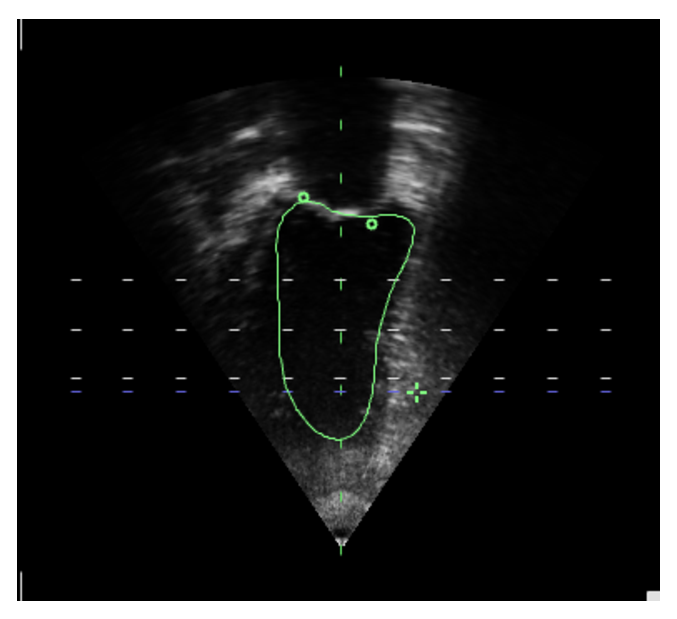
\includegraphics[width=0.9\textwidth]{LV_systole_volume_trace}}
     \caption{\label{paper1:fig:ultrasound_image}}
\end{subfigure}
\qquad
\begin{subfigure}[t]{0.25\textwidth}
    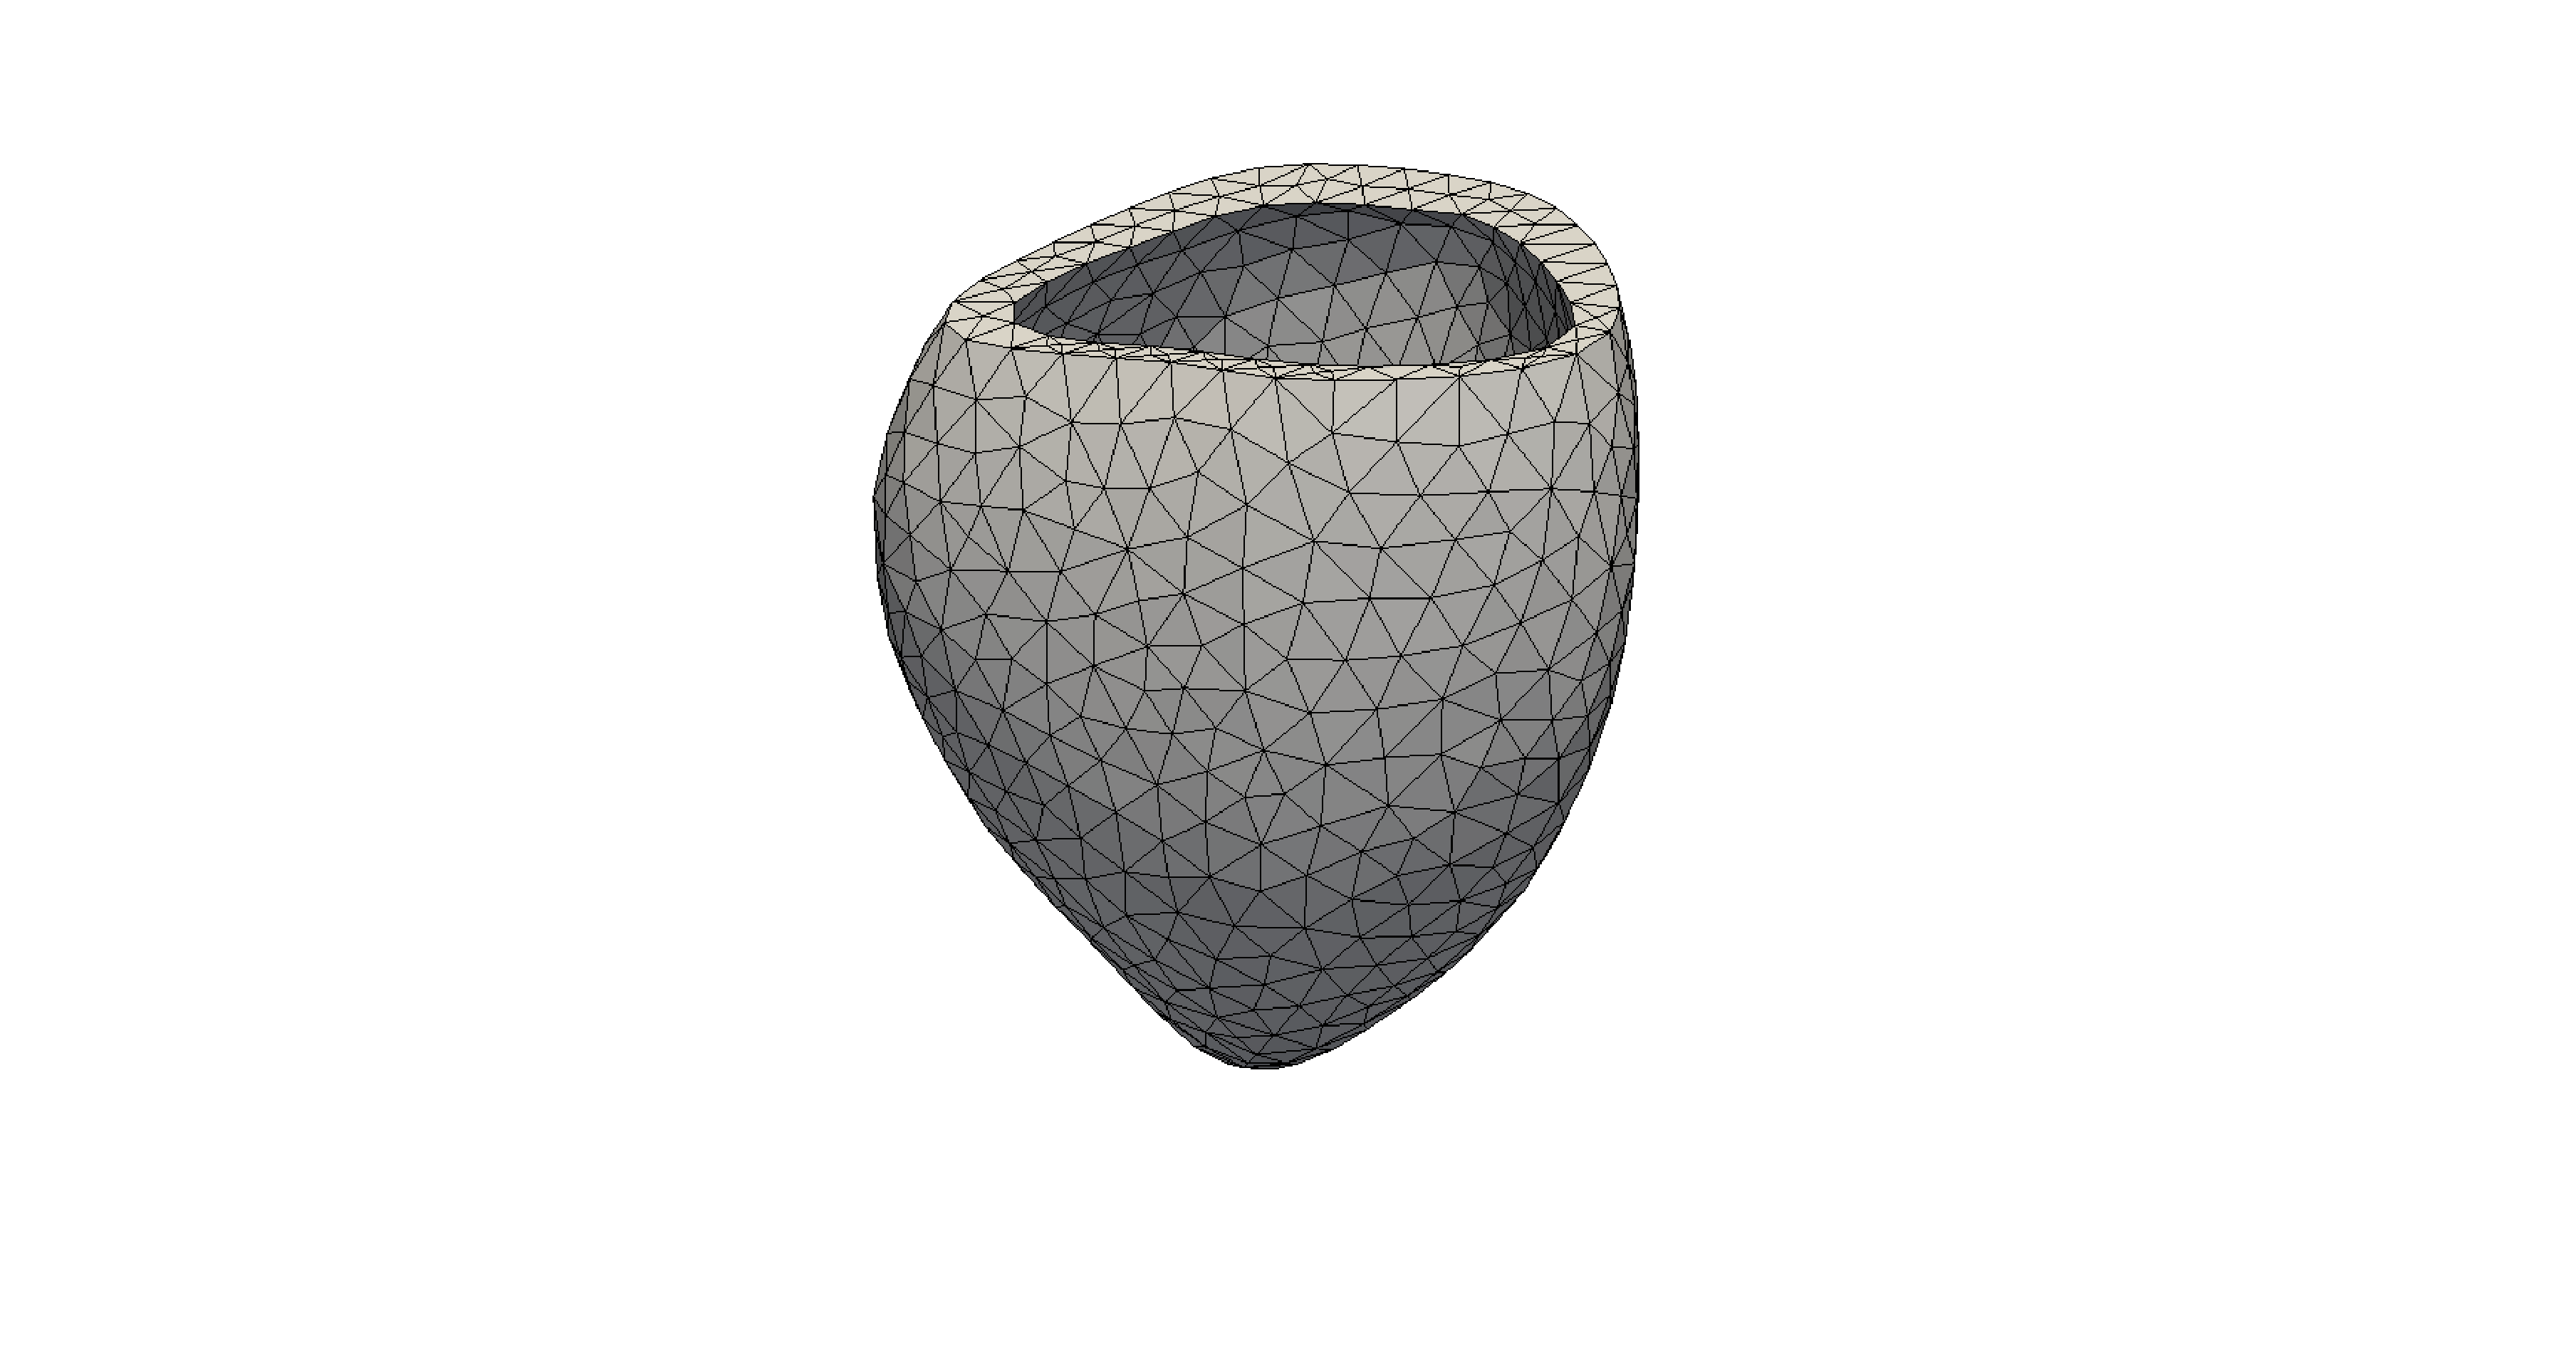
\includegraphics[width=\textwidth, trim={15cm 4cm 21cm 3cm}, clip]{mesh}
    \caption{\label{paper1:fig:compgeo_mesh}}    
\end{subfigure}
\qquad
\begin{subfigure}[t]{0.25\textwidth}
    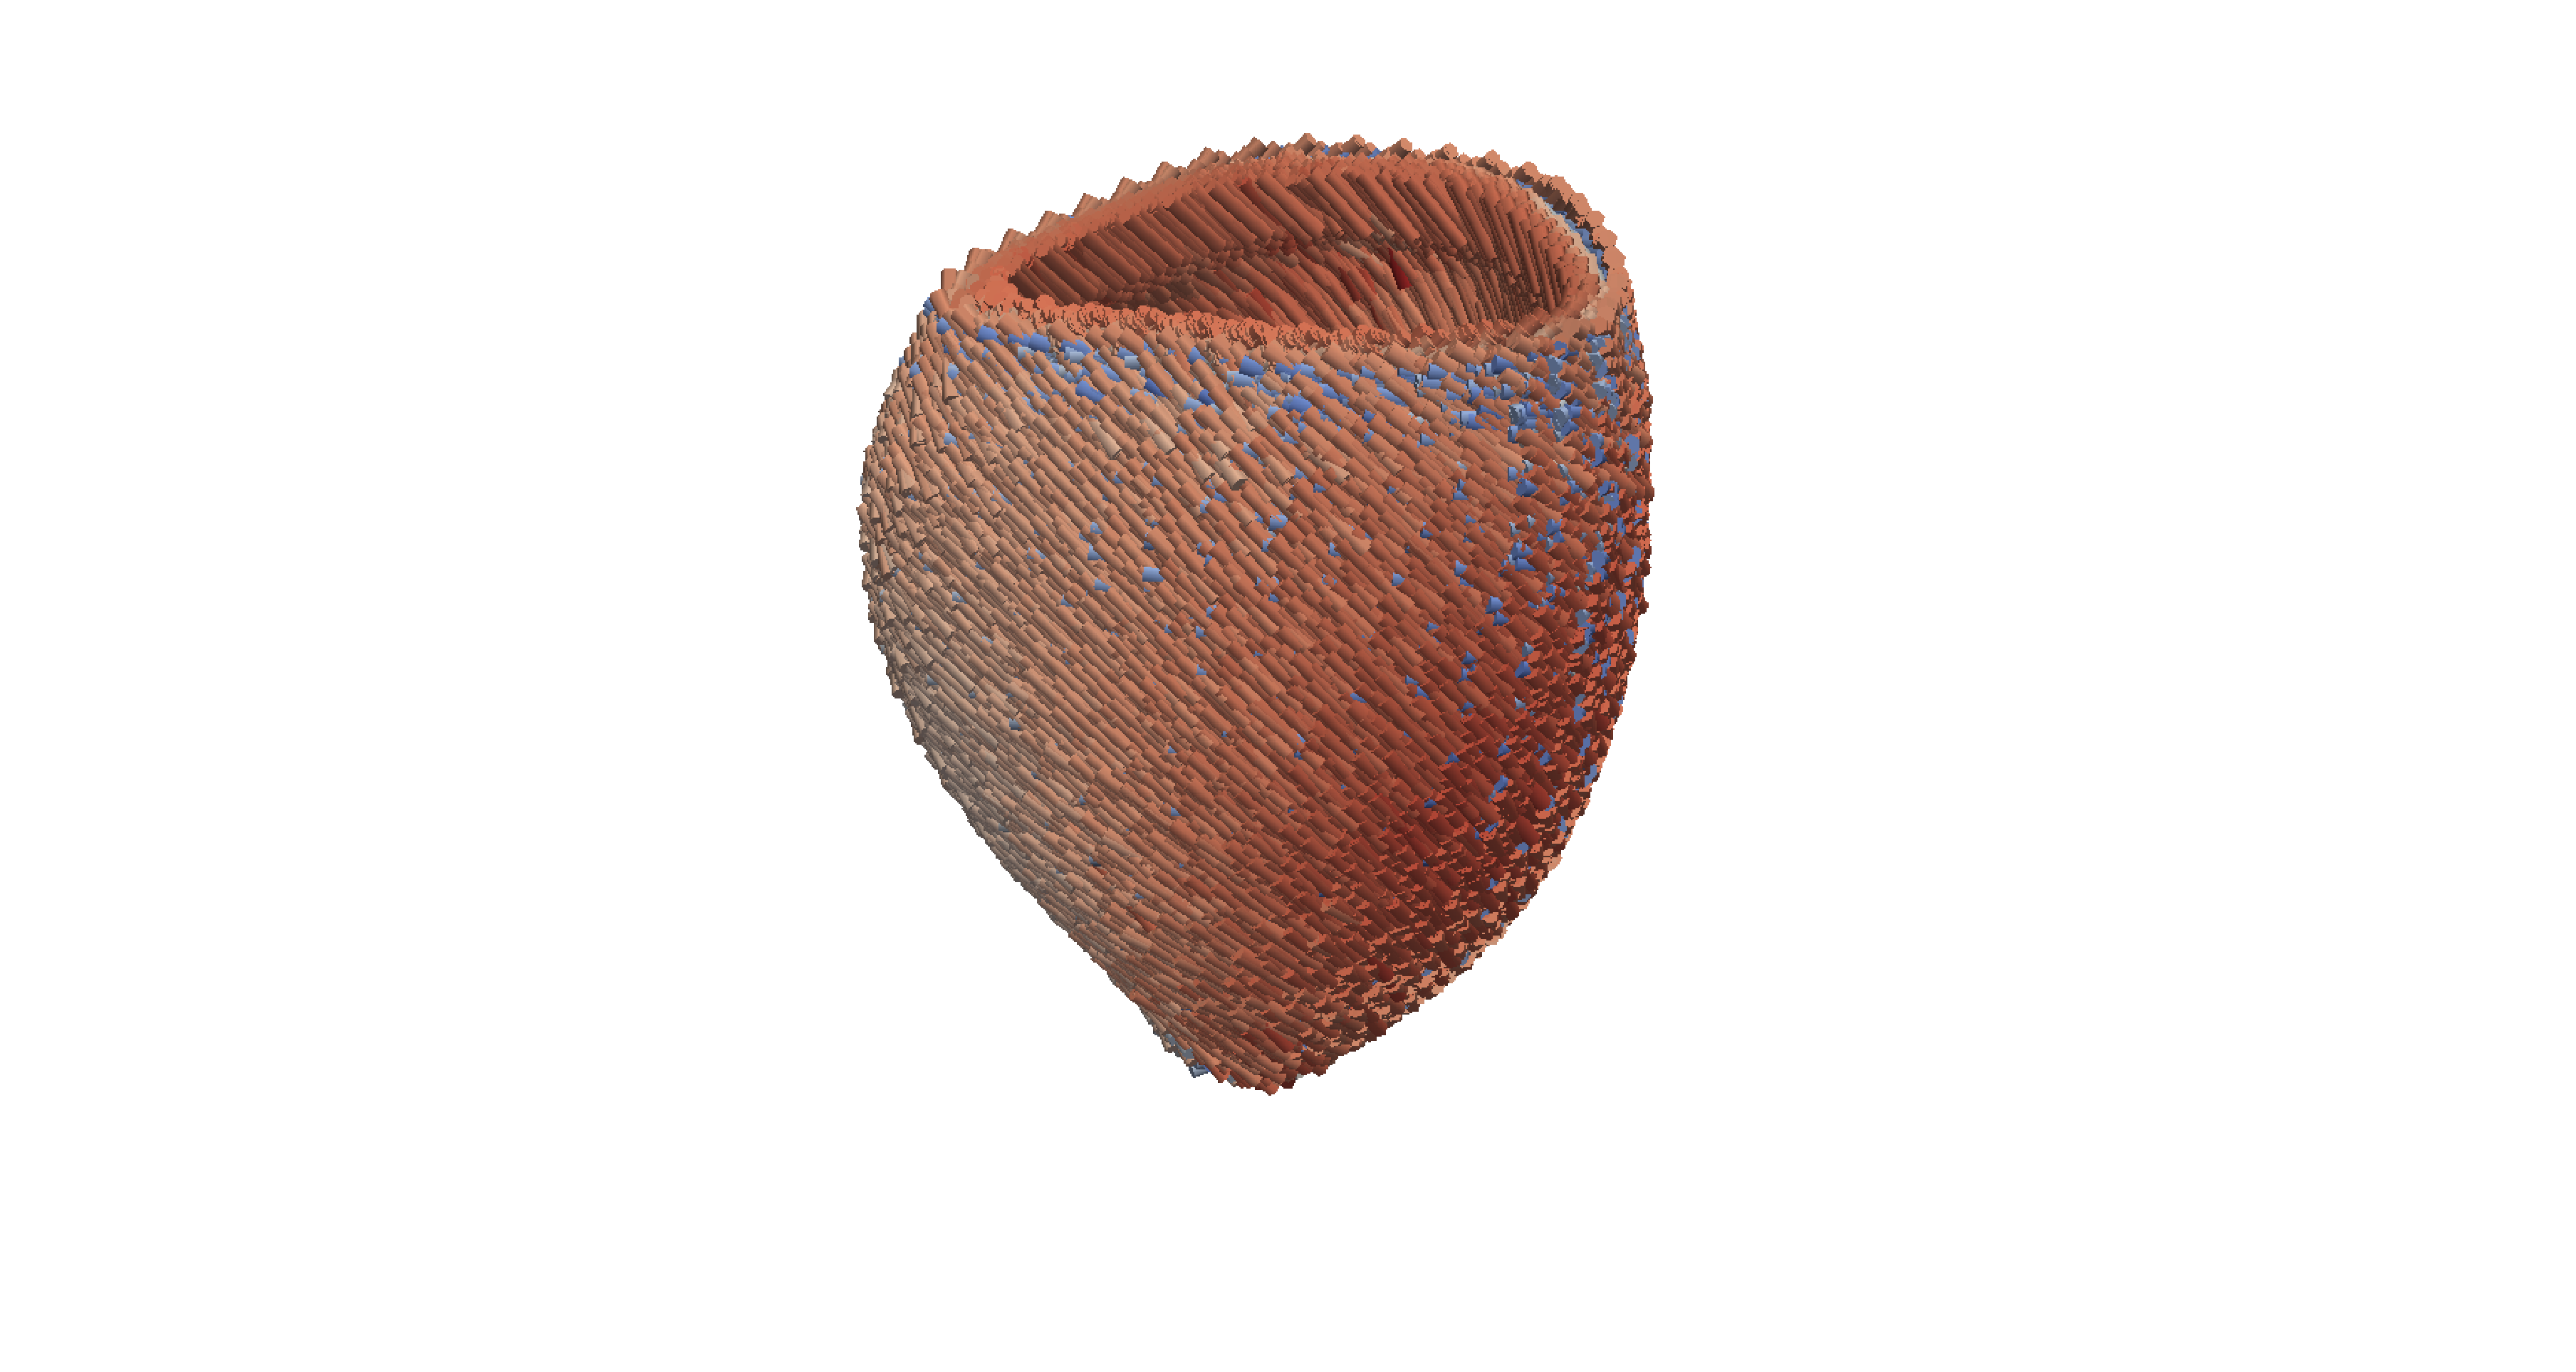
\includegraphics[width=\textwidth, trim={15cm 4cm 21cm 3cm}, clip]{fibers}
    \caption{\label{paper1:fig:compgeo_fibers}}
\end{subfigure}
\qquad
\begin{subfigure}[t]{0.25\textwidth}
    
\includegraphics[width=\textwidth, trim={15cm 4cm 21cm 3cm}, clip]{sfun}
    \caption{\label{paper1:fig:compgeo_regions}}
\end{subfigure}
\begin{subfigure}[t]{0.35\textwidth}
    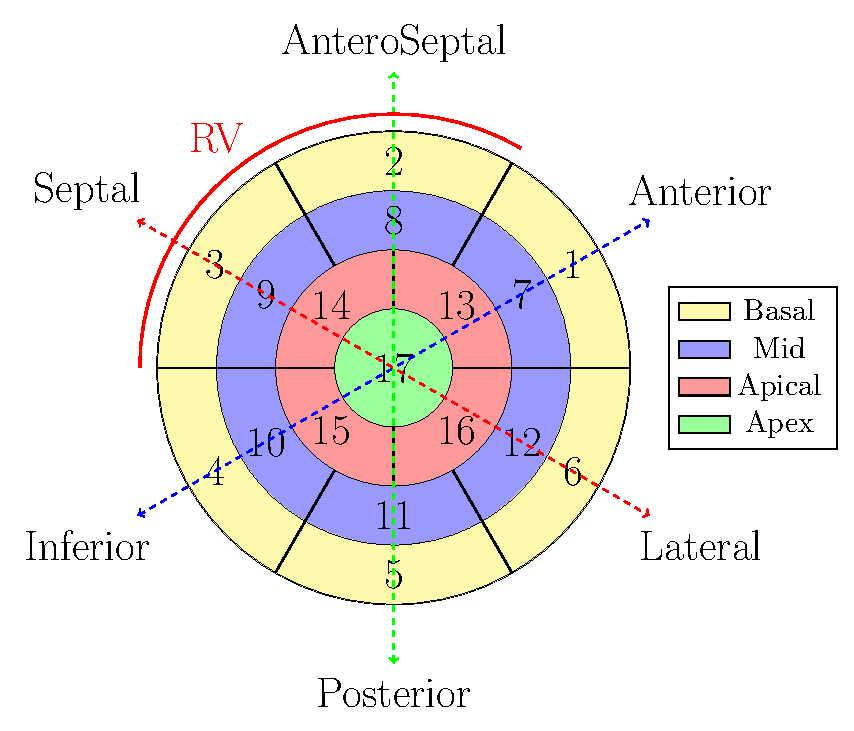
\includegraphics[width=\textwidth]{bullseye}
    \caption{\label{paper1:fig:bullseye}}
  \end{subfigure}
\caption{Ventricular geometry generation. Endo and epi-cardial surfaces 
are marked on 3-D ultrasound images. Figure (\ref{paper1:fig:ultrasound_image}) shows the endocardial 
marking for a 2-D slice of one such image. Next a computational geometry is generated
from epi and endo-cardial surfaces (\ref{paper1:fig:compgeo_mesh}), and rule based
fibers are assigned (\ref{paper1:fig:compgeo_fibers}). Finally AHA segments are assigned
to the geometry (\ref{paper1:fig:compgeo_regions}), according to the standardized scheme
(\ref{paper1:fig:bullseye}).}
\end{figure}

\subsection{Parameter Estimation}
\label{paper1:sec:paramest}
Now that we have a mathematical description of cardiac motion, along
with a personalized computational geometry and target data, we next turn to the
problem of personalizing the motion model via the estimation of the
elastic parameters and the fiber contraction. As dyssynchrony is a disease 
which primarily effects the contraction properties of the ventricle,
we focus our efforts on contraction modelling and employ a very simple
personalization of stiffness properties. That is only the parameter $a$
is optimized to fit the ventricular volumes, and the other elastic parameters
are kept fixed at the values ($a_f = 1.685, b = 9.726, b_f = 15.779$),
which were obtained from a bi-axial loading experiment 
[Table 1 row 3 of \cite{Holzapfel2009}].



Fiber contraction varies throughout the cardiac cycle, and so we estimate
the parameter $\gamma$ separately at each time measurements were taken.
Furthermore, as the contraction of the left ventricle may occur dyssynchronously, we
allow for $\gamma$ to vary in space as well as in time.


Muscle shortening is typically present in the ventricles
throughout systole and in early diastole until the muscles fully release
their contraction. During the phase of atrial systole we do not expect
muscle contraction in the ventricle, and so we set $\gamma = 0$ for
this phase. This allows us to estimate elastic properties
independently of contraction during atrial systole, and then estimate
contraction at each point in the rest of the cardiac cycle with the
material parameters fixed. In Figure~\ref{paper1:fig:pv_loop_phases} we show
the pressure-volume loop of the patient under consideration, and
highlight the phases where we estimate the contraction and elastic
parameters.

\begin{figure}[htbp]
\centering
    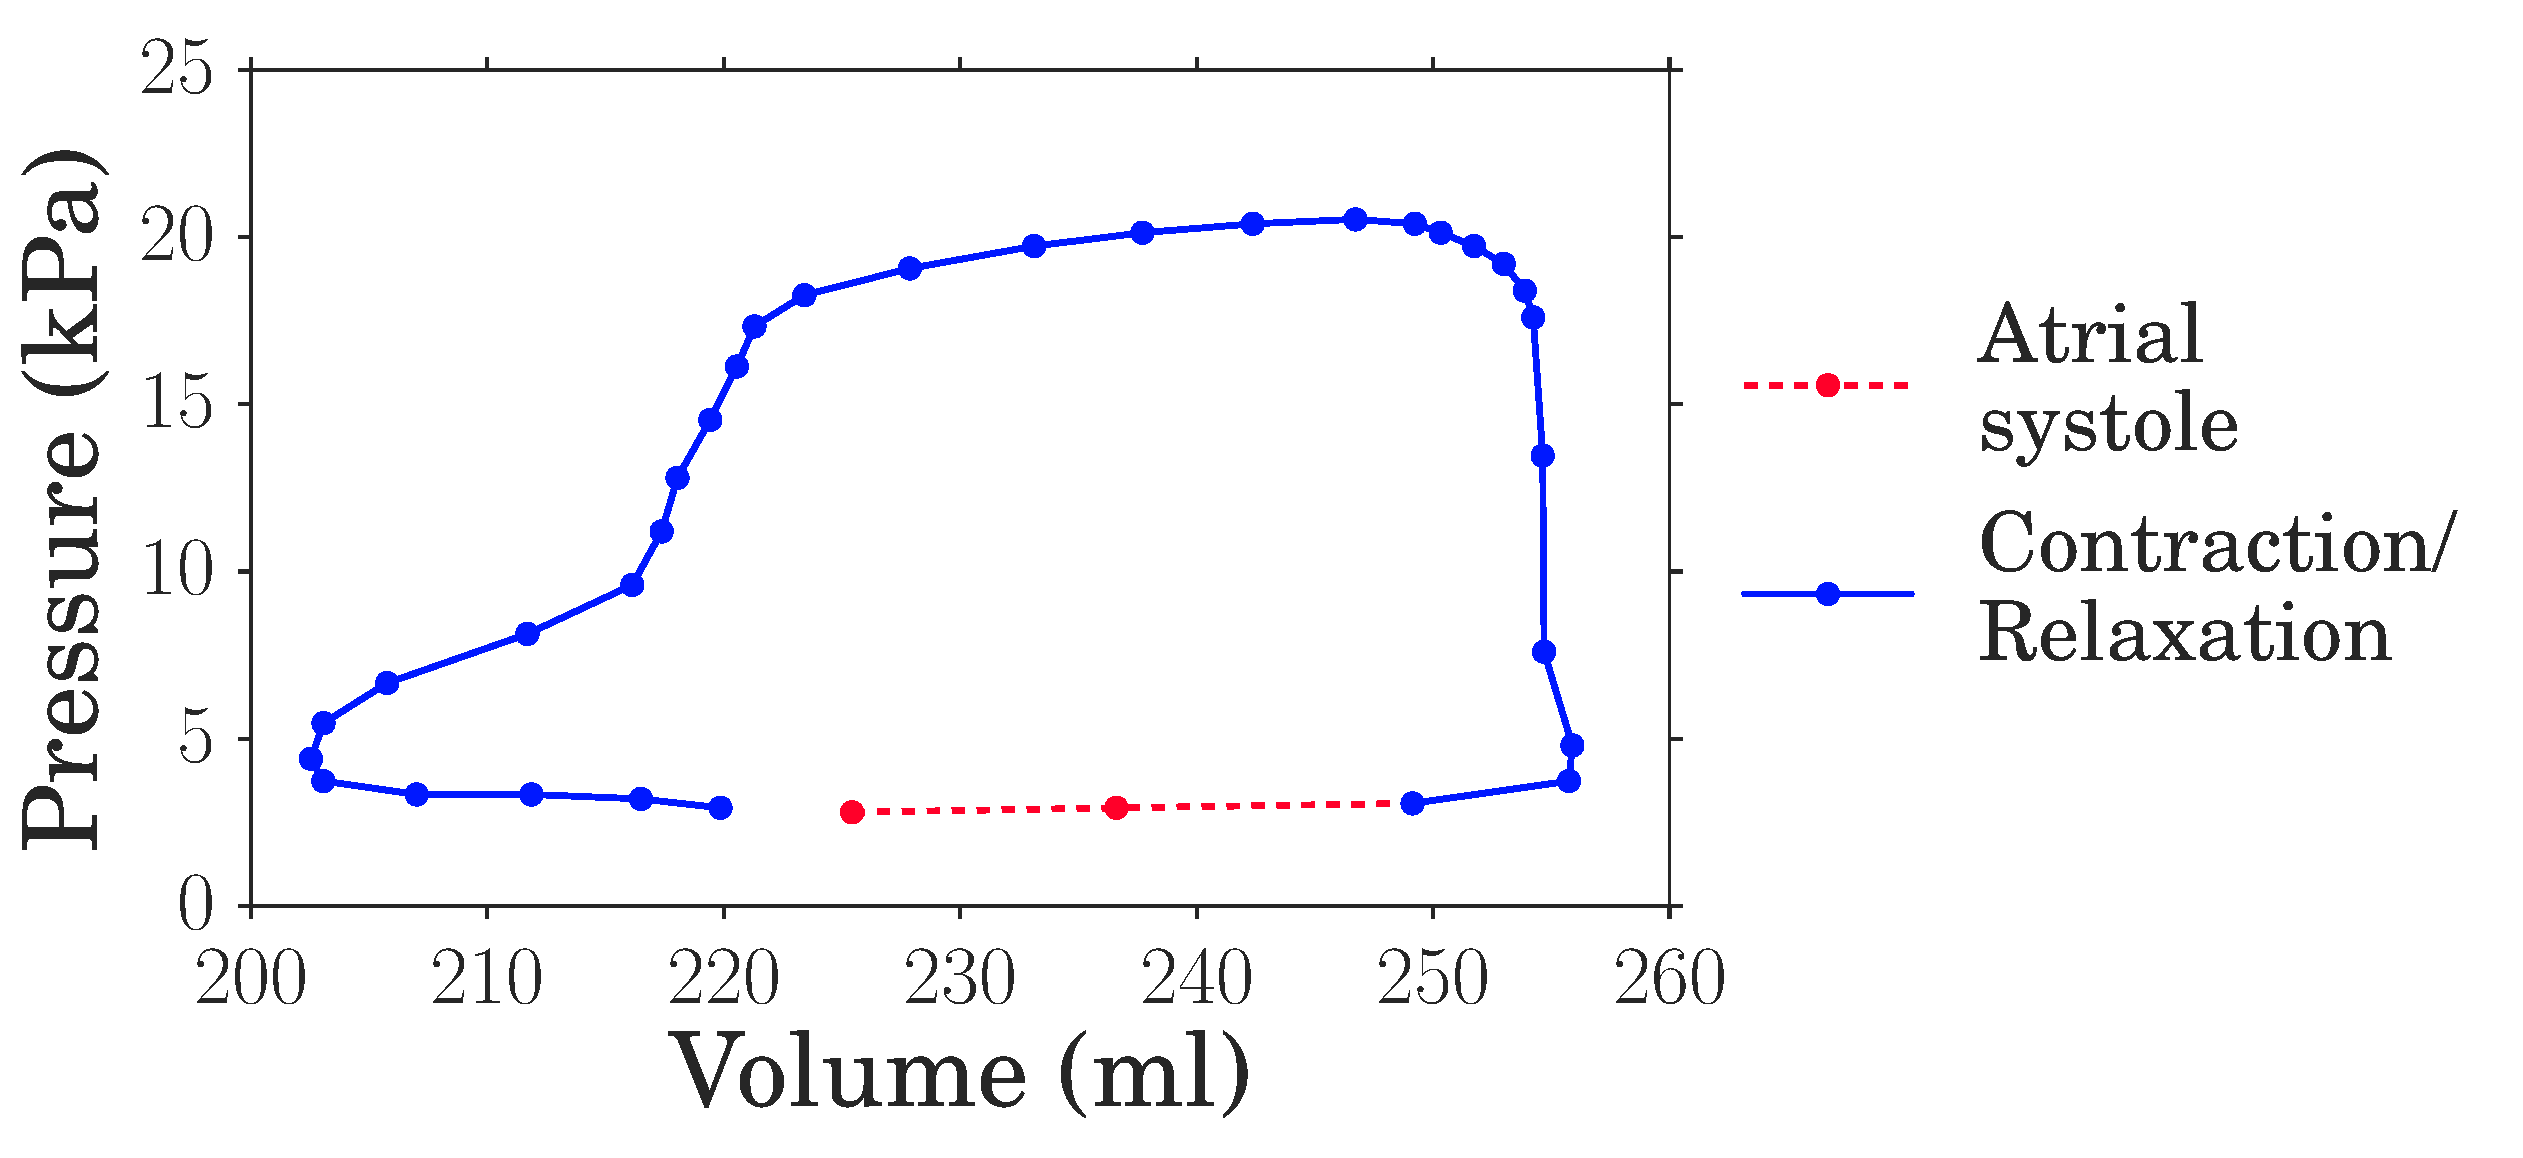
\includegraphics[width=0.8\textwidth]{patient_pv_loop}
\caption{Patient pressure-volume relationship for the left
  ventricle. Measurements in the blue solid line are used to estimate
  contraction, whereas measurements in the red dashed line are used
  to estimate elasticity. }
\label{paper1:fig:pv_loop_phases}
\end{figure}


\subsection{Definition of functionals}
\label{paper1:sec:data_func}
As described in Section~\ref{paper1:sec:clinical_measurements}, the data
available for our personalization of the wall motion model are
pressure, volume and strain measurements throughout the cardiac
cycle. The pressure measurements are included in the model as a boundary condition 
via the virtual work~\eqref{paper1:eq:work-balance},
and thus our data assimilation only needs to fit the model to
the volume and strain measurements. This requires that
we define a suitable set of functionals that quantify the
model-strain and model-volume mismatches. The personalization of the wall motion model can
then be achieved by optimizing the contraction and elastic parameters
in order to minimize the total model-data mismatch.

Let $i$ denote the index of an observed cavity volume $V^i$, or strain
$\varepsilon^i$, in the cardiac cycle. Furthermore let $j \in
\{1,..,17\}$ be the index of an AHA segment $\Omega_j$, and $k \in
\{c,r,l\}$ indicate a direction: circumferential, radial or
longitudinal, respectively. Given a measurement point $i$, we define
the model-strain mismatch
\begin{equation}
 \Istrain^i =  \sum_{j= 1}^{17} \sum_{k \in \{c,r,l\}}  \left( \varepsilon_{kj}^i -  \tilde{\varepsilon}_{kj}^i \right)^2,
\label{paper1:eq:strain_functional}
 \end{equation}
for model strain $\tilde{\varepsilon}_{kj}^i$ and measured strain
$\varepsilon_{kj}^i$. The speckle tracking software we use provides the measured strain $\varepsilon_{kj}^i$. 
This strain is regionally averaged and of Lagrangian type. In order to mimic this in our model we 
define the model strain as
\begin{equation}
\varepsilon_{kj} =  \frac{1}{|\Omega_j|}\int_{\Omega_j}  \mathbf{e}_k^T \nabla \uvec \, \mathbf{e}_k \ dx,
\label{paper1:eq:g_futhese nctional}
\end{equation}
where $\ek$ denotes a unit direction field and
$|\Omega_j|$ the volume of segment $j$.

Furthermore we also define the model-volume mismatch
\begin{equation}
  \Ivol^i  =  \left( \frac{V^i - \tilde{V}^i}{V^i} \right)^2,
\end{equation}
where the model volume is calculated by the formula
\begin{equation}
  \tilde{V}^i = -\frac{1}{3} \int_{\lvendo} (\Xvec + \uvec) \cdotp J \F^{-T} \Nvec  \ dS.
  \label{paper1:eq:vol_functional}
 \end{equation}
We note that this method of calculating the model volume depends upon
$(\Xvec + \uvec)\cdotp \Nvec = 0$ at the basal plane. These conditions hold in 
our model as the basal plane is defined with 0 longitudinal coordinate and 
longitudinal displacements are also set to 0 in this plane.

In order to have a single optimization target to describe the fit to data 
we combine the strain \eqref{paper1:eq:strain_functional} and volume
\eqref{paper1:eq:vol_functional} mismatches into one single functional
\begin{equation}
  \Idata^i(\alpha) = \alpha \Ivol^i + (1 - \alpha) \Istrain^i.
\label{paper1:eq:total_functional}
\end{equation}
Here the parameter $\alpha$ controls the relative emphasis of the parameter
estimation on volume or strain matching.

In our study we consider a high dimensional representation of $\gamma$ in order
to more accurately capture the details of a dyssynchronous contraction. However this can easily lead to
an over-parametrized problem in which many parameter combinations produce the same
functional values. In order to further constrain the optimization we introduce
a 1st order Tikohonov regularization functional
\begin{equation}
 \Ismooth^i(\lambda) = \lambda \| \nabla \gamma^i \|^2, 
 \label{paper1:eq:I_smooth}
\end{equation}
where $\|\cdotp \|$ represents the standard $L^2$ norm.
This functional discriminates between $\gamma$ parameter sets based on their smoothness.
The parameter $\lambda$ can be adjusted to control the size of the functional and hence
the relative emphasis on smoothing.

\subsection{Parameter estimation as an optimization problem}
\label{paper1:sec:param_est}
The elastic parameters of the reduced
Holzapfel-Ogden law \eqref{paper1:eq:hoa} represent the passive elastic
properties of the myocardium. We personalize these properties by
adjusting the parameter $a$ to match measured left ventricular volumes.
Mathematically this problem is formulated as
\begin{equation}
\begin{aligned}
\label{paper1:eq:opt_matparam}
& \underset{a}{\text{minimize}}
& &  \sum_{i = 1}^{\Nas} \Ivol^i \\
& \text{subject to}
& & \delta W(\plv^i, a) = 0 \quad \forall \,  i \ \in \{1,...N_{AS} \},
\end{aligned}
\end{equation}
where $\delta W$ is given by \eqref{paper1:eq:workdef}, and $\Nas =
3$ indicates the total number of measurements available in atrial
systole.

The contraction field that we seek should fit the data as closely as possible while 
also being as smooth as possible. In order to achieve this we minimize both the 
data and smoothness functionals as follows:
\begin{equation}
\begin{aligned}
\label{paper1:eq:opt_gamma}
& \underset{\gamma}{\text{minimize}}
& & \Idata^i(\alpha) + \Ismooth^i(\lambda) \\
& \text{subject to}
& &  \delta W(\plv^i, a, \gamma^i) = 0 \quad \\
&&& \gamma^i(\mathbf{X}) \in [0, 1), \ \Xvec \in \Omega.
\end{aligned}
\end{equation}
This problem is solved for every measurement point $i$ not in atrial systole.

The optimization problems \eqref{paper1:eq:opt_matparam} and \eqref{paper1:eq:opt_gamma} have two
free parameters whose values must be chosen, namely the strain-volume
weighing $\alpha$ and the regularization $\lambda$. The value of $\lambda$ can be expected to influence the trade-off
between the optimized values of the data functional $\Idata^i$ and the regularization functional
$\Ismooth^i$. Similarly $\alpha$ can be expected to influence the trade-off between $\Istrain^i$
and $\Ivol^i$. In our study we choose the values of $\alpha$ and $\lambda$ by examining their effects on the functionals
that they weigh. The choices we made are further described in Section~\ref{paper1:sec:a_l_choice}

The spatial resolution of the parameter $\gamma$ affects the amount of detail
that can be captured by the model and simultaneously
the number of variables that need to be optimized. We therefore test 3 different resolutions of $\gamma$.
The lowest resolution, ``scalar'', is simply a single global value.  The next resolution
is ``regional'', and consists of a separate value for each of the 17 AHA zones. Finally, the highest resolution
we consider is ``P1'' and consists of a separate value at each of the vertices of the mesh,
with a linear interpolation between vertices. Using our ventricular mesh, a P1 resolution of $\gamma$ has 1262 separate variables.


\subsection{Implementation of mechanics and optimization solvers}
For the numerical solution of the work balance equation~\eqref{paper1:eq:work-balance} we employ a
Galerkin finite element method with Taylor-Hood tetrahedral
elements~\cite{hood1974navier}; that is, a continuous piecewise
quadratic representation of the displacement field and a continuous
piecewise linear representation of the pressure field.  

The software implementation of our finite element method is based on
the package FEniCS~\cite{LoggMardalEtAl2011a}, which automatically
generates matrix and vector assembly code from a symbolic
representation of the work balance equation~\eqref{paper1:eq:work-balance}.
The resulting nonlinear systems were solved using the PETSc
implementation of a Newton trust region algorithm~\cite{PETScPackage},
while the inner linear solves were handled by a distributed memory
parallel LU solver~\cite{lidemmel03}.

To solve the optimization problems \eqref{paper1:eq:opt_matparam} and
\eqref{paper1:eq:opt_gamma}, we apply a sequential quadratic programming
algorithm (SQP)~\cite{kraft1988software}. This algorithm requires the
derivatives of the function to be optimized, which in our case are the
gradients of the mismatch functionals in
problems~\eqref{paper1:eq:opt_matparam} and \eqref{paper1:eq:opt_gamma} with respect
to $a$ and $\gamma$ respectively. These gradients are
automatically computed by solving a machine derived adjoint equation via the
software framework dolfin-adjoint~\cite{farrell2013automated}.

In addition to gradients, the SQP algorithm requires evaluations of
the mismatch functionals for given values of the control variables,
which again relies on the solution of the work balance
equation~\eqref{paper1:eq:work-balance}. In the case of
problem~\eqref{paper1:eq:opt_gamma}, the control variable is $\gamma$, which
has a large influence on the solution of \eqref{paper1:eq:work-balance}.
Numerical solution of \eqref{paper1:eq:work-balance} by Newton's method
depends upon having a good initial guess, which in our case are the
values of the mechanical state variables, $\uvec, p$, resulting from
the previous solve of \eqref{paper1:eq:work-balance}. If the value of
$\gamma$ differs too greatly from one solve to the next the Newton
algorithm might fail due to the root of the system being too far away
from the initial guess. To avoid this problem we make use of a
homotopy procedure that moves from one value of $\gamma$ to the next
in small increments, and solves \eqref{paper1:eq:work-balance} each time the
value of $\gamma$ is changed.  This procedure is presented as
Algorithm~\ref{paper1:alg:homotopy-newton} and is similar to the one found
in~\cite{pezzuto2014orthotropic}. 

All algorithms, solvers and relevant data are
publicly available online \cite{OurPackage}.

\begin{algorithm}
\caption{Max Increment Homotopy Newton Solver}
\label{paper1:alg:homotopy-newton}
  \begin{algorithmic}
   \State \emph{Initial Variables}
   \State $\begin{array}{ll}
    \quad \uvec_{prev} & \quad \quad \quad  \mbox{Previous displacement field} \\
    \quad p_{prev} & \quad \quad \quad  \mbox{Previous tissue hydrostatic pressure field} \\
    \quad \gamma_{next} & \quad \quad \quad  \mbox{Desired tissue contraction field} \\
    \quad \delta \gamma_{max} & \quad \quad \quad  \mbox{Maximum change in a component per Newton solve}
   \end{array}$

   \\
   \State \emph{Set}
   \State \quad $\gamma_0 = \gamma_{prev}$
   \State \quad $\uvec_0 = \uvec_{prev}$
   \State \quad  $p_0 = p_{prev}$
   \State \quad  $M = \left \lceil \frac{\|\gamma_{next} - \gamma_{prev}\|_{\infty}}{\delta \gamma_{max}} \right \rceil$
   \State \quad $\delta \gamma = \frac{1}{M}(\gamma_{next} - \gamma_{prev})$
   \\
   \State \emph{Use Newton's method $M$ times with fixed increment $\delta \gamma$}
   \For{$i \in \{1...M\}$}
      \State $\gamma_i = \gamma_{i -1} + \delta \gamma$
      \State Initialize Newton solver with $\uvec_{i -1}, p_{i -1}$
      \State Solve $\delta W(\uvec_i, p_i, \gamma_i) = 0$ for $\uvec_i, p_i$
   \EndFor
   \State Output $\uvec_i, p_i$
  \end{algorithmic}
\end{algorithm}

\subsection{Error Estimation}

The optimization functionals introduced in Section~\ref{paper1:sec:data_func} are defined 
separately for each measurement
point. For the purposes of evaluating goodness of fit over the entire cardiac cycle
we consider metrics that are averaged over measurement points. Furthermore we 
relate errors to the sizes of the data 
for ease of interpretation. In the case of the model-volume error we introduce the volume metric
\begin{equation}
\overline{I}_{\text{vol}} = \frac{ \| V^i - \tilde{V}^i \|_{\ell^1}}{ \| V^i \|_{\ell^1}}
\label{paper1:eq:average_volume}
 \end{equation}
where the $\ell^1$ norm is taken with respect to the measurement point index $i$.
Furthermore we consider two average strain metrics
\begin{align}
\Istrainavg &= \frac{1}{51} \sum_{j= 1}^{17} \sum_{k \in \{c,r,l\}}
\frac{\| \varepsilon^i_{k,j} -  
\tilde{\varepsilon}^i_{k,j} \|_{\ell^1} }{ \| \varepsilon^i_{k,j} \|_{\ell^1}}, \\
\Istrainrelmax &=  \frac{1}{51} \sum_{k \in \{c,r,l\}}
 \frac{\sum_{j= 1}^{17} \| \varepsilon^i_{k,j} 
 -  \tilde{\varepsilon}^i_{k,j} \|_{\ell^1}}{ \max_j \| \varepsilon^i_{k,j} \|_{\ell^1}}.
\label{paper1:eq:average_strain}
\end{align}
Here $N$ specifies the number of measurement points used in the
optimization, and the factor $51$ is $17 \times 3$,
the number of AHA segments times the number of strain measurements per segment. 
The first metric considers relative differences between norms, whereas the second relates 
errors norms to the maximum
strain norm over all segments. This second metric emphasizes larger features in 
the strain curves more heavily, and deemphasizes
small scale features such as noise.

Similarly to the average data errors introduced above we also introduce a smoothness 
metric that is averaged across measurement points
\begin{equation}
\overline{I}_{\text{smooth}} = \frac{1}{N}\sum_{i = 1}^N \Ismooth^i, \\
\end{equation}
and a combined data metric based on the strain and volume metrics
\begin{equation}
  \Idataavg = \Ivolavg + \Istrainavg.
\label{paper1:eq:total_functional}
\end{equation}

Finally we also define an error metric for a synthetic
data test of the contraction optimization \eqref{paper1:eq:opt_gamma}. In this
test a contraction field $\gamma_{\text{ground}}$ is chosen and 
synthetic data is generated from the 
mechanics model. This data is then used to calculate a
reproduction of the contraction $\gamma_{\text{repr}}$. 
In order to compare the ground truth and reproduced contraction 
fields we employ a relative $L^2$ norm
\begin{equation}
  \| \epsilon_{\gamma} \|_{\text{avg}} = \frac{1}{N} \sum_{i = 1}^{N}  \frac{\| \gamma_{\text{repr}}^{i} -
  \gamma_{\text{ground}}^{i} \|_{L^2}}{ \| \gamma_{\text{ground}}^{i} \|_{L^2}}.
\label{paper1:eq:error_gamma}
\end{equation}

\section{Numerical Experiments}
\label{paper1:sec:num_results}
In this section we present the results of our numerical experiments.
We first estimate the parameter $a$ using volume measurements in atrial systole.
We then test the estimation of contraction $\gamma$ using synthetic data generated
by the wall motion model. This gives an idea of how well the algorithm
can perform under idealized circumstances.  Next, we
carry out the contraction estimation using the clinical strain and volume data.
Finally, we consider lower resolution representations of $\gamma$, and compare 
the resolutions based on computational expense and data matching capability.

In all of the experiments below, optimizations were terminated if the
difference between the value of the mismatch in the current and
previous iteration was less than $10^{-9}$ for the passive material
parameter optimization and $10^{-6}$ for the contraction
parameter optimization or if the
SQP algorithm was not able to further reduce the mismatch value.
In the active parameter optimization the SQP
algorithm was initialized with the value of $\gamma$ from the previous
measurement point in the cardiac cycle. 

In order to obtain convergence of Newton's method for the solution of
the virtual work equation~\eqref{paper1:eq:work-balance}, we set $\delta
\gamma_{max} = 0.02$ in the homotopy Newton solver
(Algorithm~\ref{paper1:alg:homotopy-newton}), and 
limit $\gamma$ to the interval $[0, 0.9]$. In the cases that Newton's
method did not converge, $\delta \gamma_{max}$ was halved until convergence was obtained. 

Strains were calculated with respect to the measurement point defined
as start of atrial systole, as the reference geometry taken from the
image corresponding to this point was assumed to be stress and strain
free. Similarly, pressures for the clinical data were adjusted
downward by the pressure measured at the start of atrial systole, 2.8
kPa, so that the adjusted start of atrial systole pressure was 0, and
therefore compatible with the stress free assumption.

The value of the basal spring-constant was set to $k = 1.0$ kPa. This allowed for some
motion in the basal plane,
and was shown in a sensitivity analysis (see Appendix~\ref{paper1:sec:k_sense})
to give optimal $\gamma$ values
whose spatial average is close to that obtained with a completely fixed boundary.

\subsection{Estimation of elastic parameter $a$}
\label{paper1:sec:elasticparam}
An estimate of the parameter $a$ was obtained by minimizing the mismatch between
model derived and clinically measured volumes in atrial systole,
as described in \eqref{paper1:eq:opt_matparam}. The optimal $a$ value obtained was $0.435$, 
with goodness of fit $\overline{I}_{\text{vol}} = 0.0035$.
The same optimal $a$ value was obtained from 8 randomly chosen starting points
between 0 and 45.


\subsection{Synthetic dataset creation}

\label{paper1:sec:data_synthetic}
In order to evaluate the performance of our contraction estimation
method \eqref{paper1:eq:opt_gamma} under idealized conditions we  
have performed synthetic data tests. The data for these tests was
constructed by solving the virtual work 
equation~\eqref{paper1:eq:work-balance} for a given set of elastic parameters
 $(a, a_f, b, b_f)$, contraction $\gamma$, and cavity pressures.
The $a$ parameter was set to $0.435$, as obtained previously by
fitting the model to the patient atrial systolic volume data. The
other three elastic parameters were fixed to the values mentioned in Section~\ref{paper1:sec:paramest}.
The contraction $\gamma$ was chosen to be a wave 
with Gaussian shape and P1 resolution traveling along the longitudinal axis.

Eight points of measurement were used in the synthetic tests. This was
fewer than the number of in-vivo  
measurement points, which allowed for faster computations. The
pressure values that were chosen  
for the synthetic measurement points
can be seen in Figure~\ref{paper1:fig:synthetic_gammafields}. These pressures start at 0, 
increase to the maximum atrial systole pressure 
that was measured in-vivo and then decrease linearly back to 0. 


For the synthetic strain data we considered three different cases. The
first case consisted of the displacement  
gradient tensor defined over the entire ventricular geometry. Next we
considered regionally averaged values of the 
diagonal components of the displacement gradient. The regional averaging mimics the
strain curves generated by the speckle tracking software.  
Finally we consider 30 noisy realizations of the regional strain
curves. The noise that was added to these curves was estimated 
from the drift values of the in-vivo strain and is described in
Appendix~\ref{paper1:sec:strain_noise_est}.


\subsection{Choice of functional weights $\alpha$ and $\lambda$}
\label{paper1:sec:a_l_choice}
The optimization functional weights $\alpha$ and $\lambda$ were chosen based on
trial optimizations using the synthetic and in-vivo datasets. The strains in the synthetic
data were regionally averaged and noisy.
In these trials we first set $\lambda = 0$ and tested $\alpha$ values
ranging from 0 to 1.0 in increments of 0.1, in addition to the values
0.95, 0.99, 0.999, and 0.9999.
For each level of $\alpha$ we recorded the values of the
fit metrics, $\Ivolavg$ 
and $\Istrainavg$, and plotted them against each
other (Figure~\ref{paper1:fig:lcurves}). Based on the plot 
we chose $\alpha = 0.95$ as this value gave a good balance between
volume and strain matching.  
With the value of $\alpha$ fixed to $0.95$ we tested $\lambda$
from $10^{-6}$ to $100.0$ in increasing powers of 10.
The effect of the choice of $\lambda$ on the smoothness and data functionals
is shown in Figure~\ref{paper1:fig:lcurves}. Based on this plot we selected points
that gave near optimal fit values with a high level of smoothness. 
These points were $\lambda = 1.0$ for the synthetic case
and $\lambda = 0.01$ for the patient case.



\subsection{Contraction estimation with synthetic data}
\label{paper1:sec:results_synthetic}
Using the synthetic datasets described in Section \ref{paper1:sec:data_synthetic} as a target we 
calculated optimized contraction fields. All elastic parameters 
were kept fixed throughout the optimization so that the test was restricted to
the contraction field.
We quantified the error in the reproduction of $\gamma$ using P1
resolution for the three cases of strain. Errors in the relative norm, $\| \epsilon_{\gamma} \|_{\text{avg}}$,
were 0.033 for the full displacement gradient tensor and 0.227 for the 
regionally averaged diagonal of the displacement gradient without noise. The average error
for the 30 noisy regionally averaged cases was 0.224 with a standard deviation of 0.009.
We note that the reproduction error was lowest for the full clean strains, 
and an order of magnitude higher
for the regional clean and regional noisy strains. We also note that the 
reproduction error using regional clean strains was very
close to the average reproduction error from the 30 regional noisy strains.
The maximum error for all three cases of strain occured in the apex, 
and was 0.06, 0.0701, 0.0724 for the full, regional clean and regional noisy cases
respectively.



For the case of the full clean strains we have plotted the 
reconstructed contraction field alongside the ground truth in
Figure~\ref{paper1:fig:synthetic_gammafields}. 
We note that the ground truth and reproduction appear very similar. In
order to visualize the effect of the  
noise in strain on the optimized contraction field we
plotted the mean and standard deviation of the 30 synthetic strain curves,
and mean and standard deviation of the average of the contraction field 
resulting from the 30 strain curves. Both of these plots are
restricted to the anterior basal segment and are shown in Figure
\ref{paper1:fig:noisy_strain_curve}. We note that the effect of the noise on
the average contraction field is minimal.


\begin{figure}[htbp]
\centering
\begin{subfigure}[t]{0.49\textwidth}
  \caption*{\Large{Synthetic}}
     \includegraphics[width=0.845\textwidth]{{l_curve_fixed_lambda_0.0_synth_w_noise}.eps}
\end{subfigure}
\begin{subfigure}[t]{0.49\textwidth}
  \caption*{\Large{Patient}}
  \includegraphics[width=\textwidth]{{l_curve_fixed_lambda_0.0_patient}.eps}
\end{subfigure}
\begin{subfigure}[t]{0.49\textwidth}
     \includegraphics[width=0.845\textwidth]{{l_curve_fixed_alpha_0.95_synth_w_noise}.eps}
\end{subfigure}
\begin{subfigure}[t]{0.49\textwidth}
  \includegraphics[width=\textwidth]{{l_curve_fixed_alpha_0.95_patient}.eps}
\end{subfigure}
\caption{Trade-off curves for various $\alpha$ and $\lambda$ values
  used in model personalization with synthetic strain data and in-vivo patient data.
  The synthetic strains are noisy and regionally averaged. The contraction parameter is represented 
  at P1 resolution.
  Top:
  optimal strain mismatch \eqref{paper1:eq:average_strain} versus average volume mismatch \eqref{paper1:eq:average_volume} 
  for a range of $\alpha$ values and $\lambda = 0.0$.  Bottom: Total data mismatch
  versus contraction gradient size for a range of $\lambda$ values
  and $\alpha = 0.95$.}
\label{paper1:fig:lcurves}
\end{figure}
% 
\begin{figure}[htbp]
  \begin{subfigure}[t]{0.5\textwidth}
    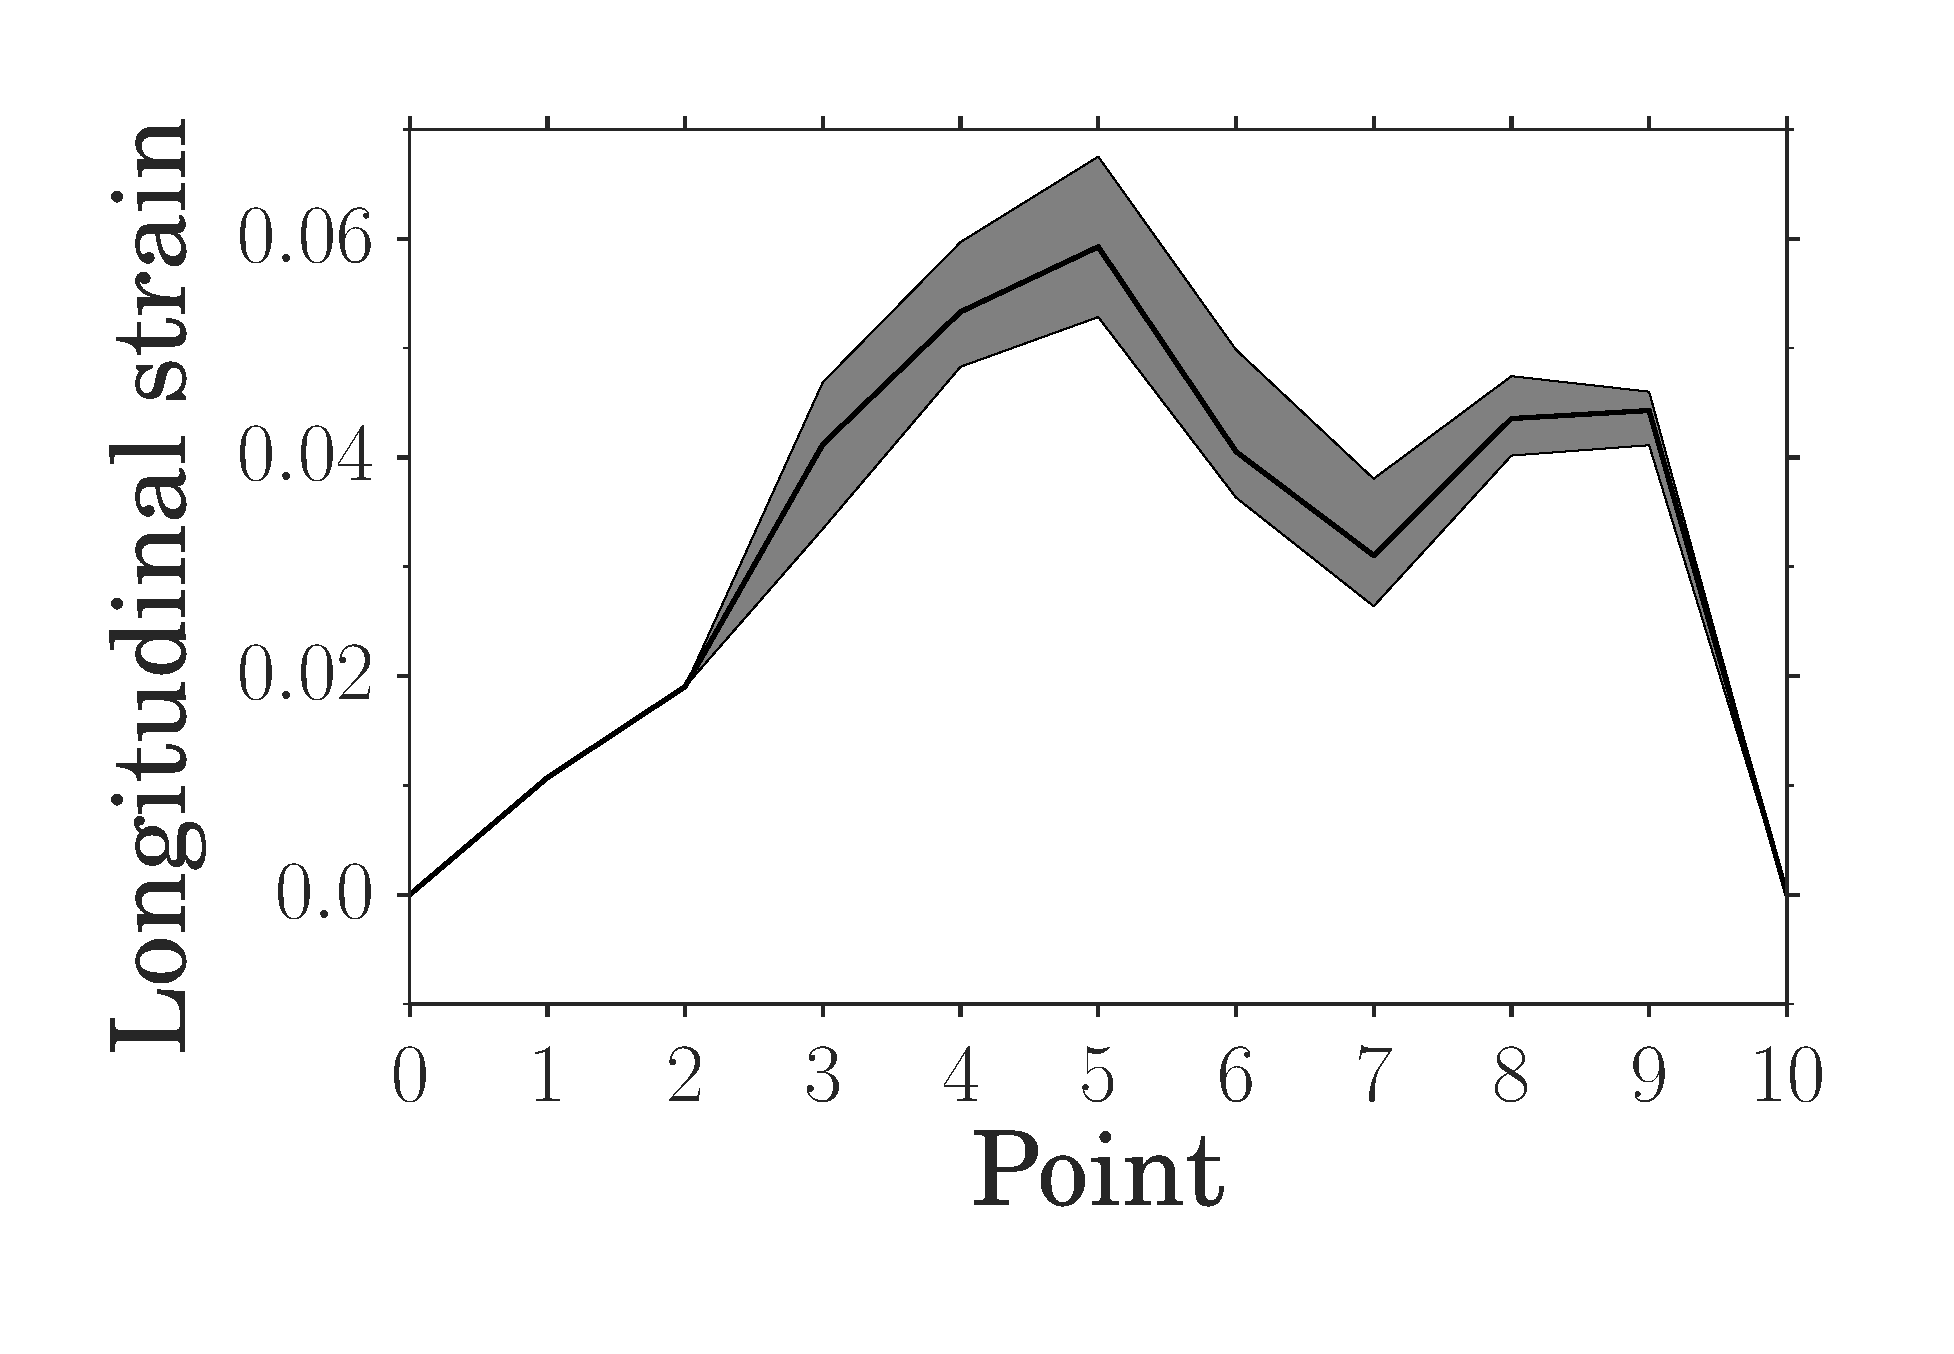
\includegraphics[width=\textwidth]{noisy_strain_region_1_ground.eps}
  \end{subfigure}
  \begin{subfigure}[t]{0.41\textwidth}
    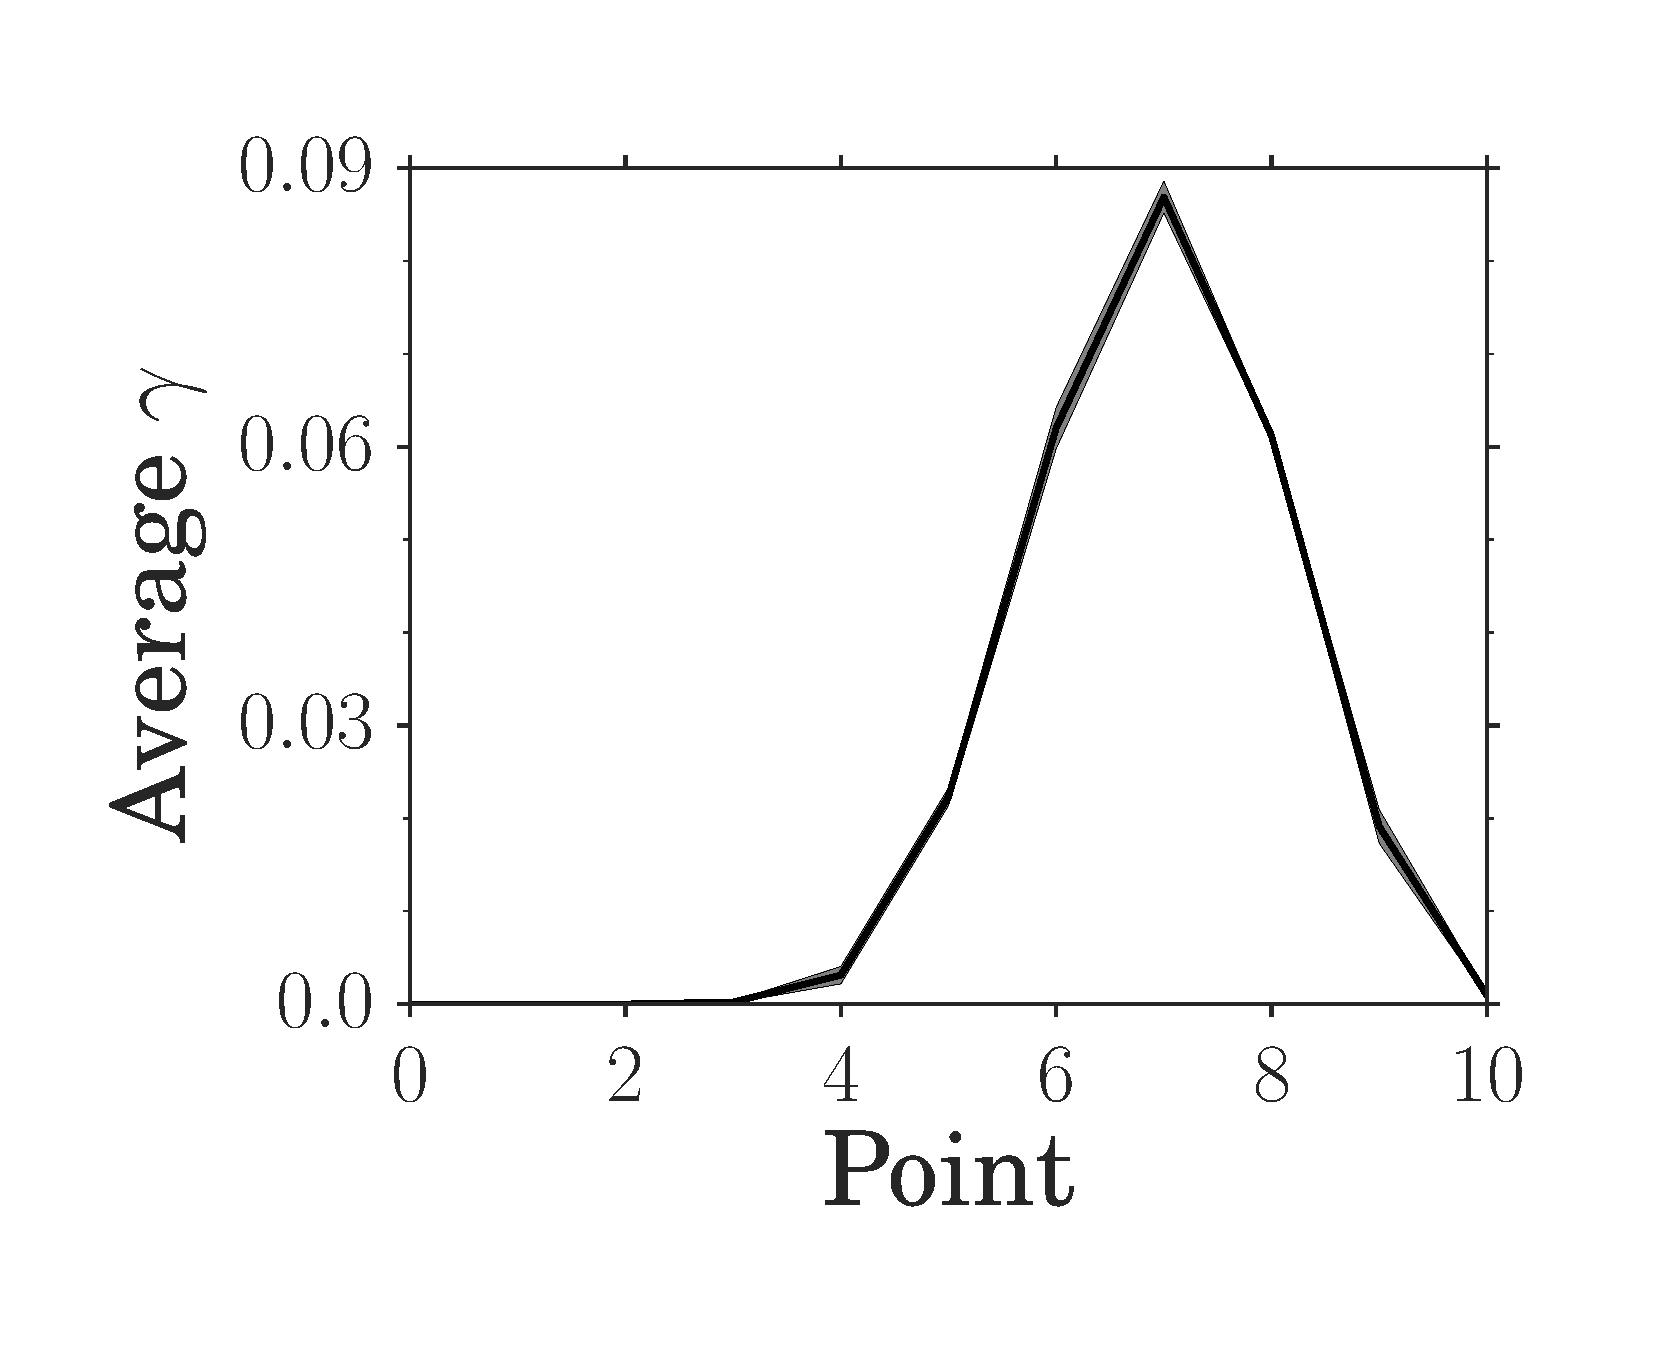
\includegraphics[width=\textwidth]{mean_gamma_region_1_synth_w_noise.eps}
  \end{subfigure}
\caption{
On the left are the mean (solid line) and standard deviation (highlighted area) of 30
synthetic longitudinal strain curves in the anterior basal segment corrupted by Gaussian noise.
On the right are the mean and standard deviations of
$\gamma$ averaged over the same segment.}
\label{paper1:fig:noisy_strain_curve}
\end{figure}


\begin{figure}[htbp]
 \includegraphics[width=1.0\textwidth]{synthetic_gamma_snapshots.eps}
 \caption{Lateral view of the ground truth and reconstructed contraction fields at 7 measurement points during
  the synthetic data test. The target for the optimization is the full strain field with no noise.
 At each pressure the reconstruction is displayed on the left and the ground truth on the right.}
\label{paper1:fig:synthetic_gammafields}
 \end{figure}

\subsection{Contraction estimation with in-vivo data}
\label{paper1:sec:results_clinical}

Using the in-vivo data described in
Section~\ref{paper1:sec:clinical_measurements} as a target, we calculated optimized contraction 
fields at P1 resolution. These contraction fields are shown in
Figure~\ref{paper1:fig:snap_shots}. We note that the value of the contraction varies significantly in space and time.
A comparison of the estimated to the measured PV loop is shown in Figure~\ref{paper1:fig:pv_match}. Optimized
and measured strains are compared in Figure~\ref{paper1:fig:strain_match}.

\begin{figure}[htbp]
\centering
  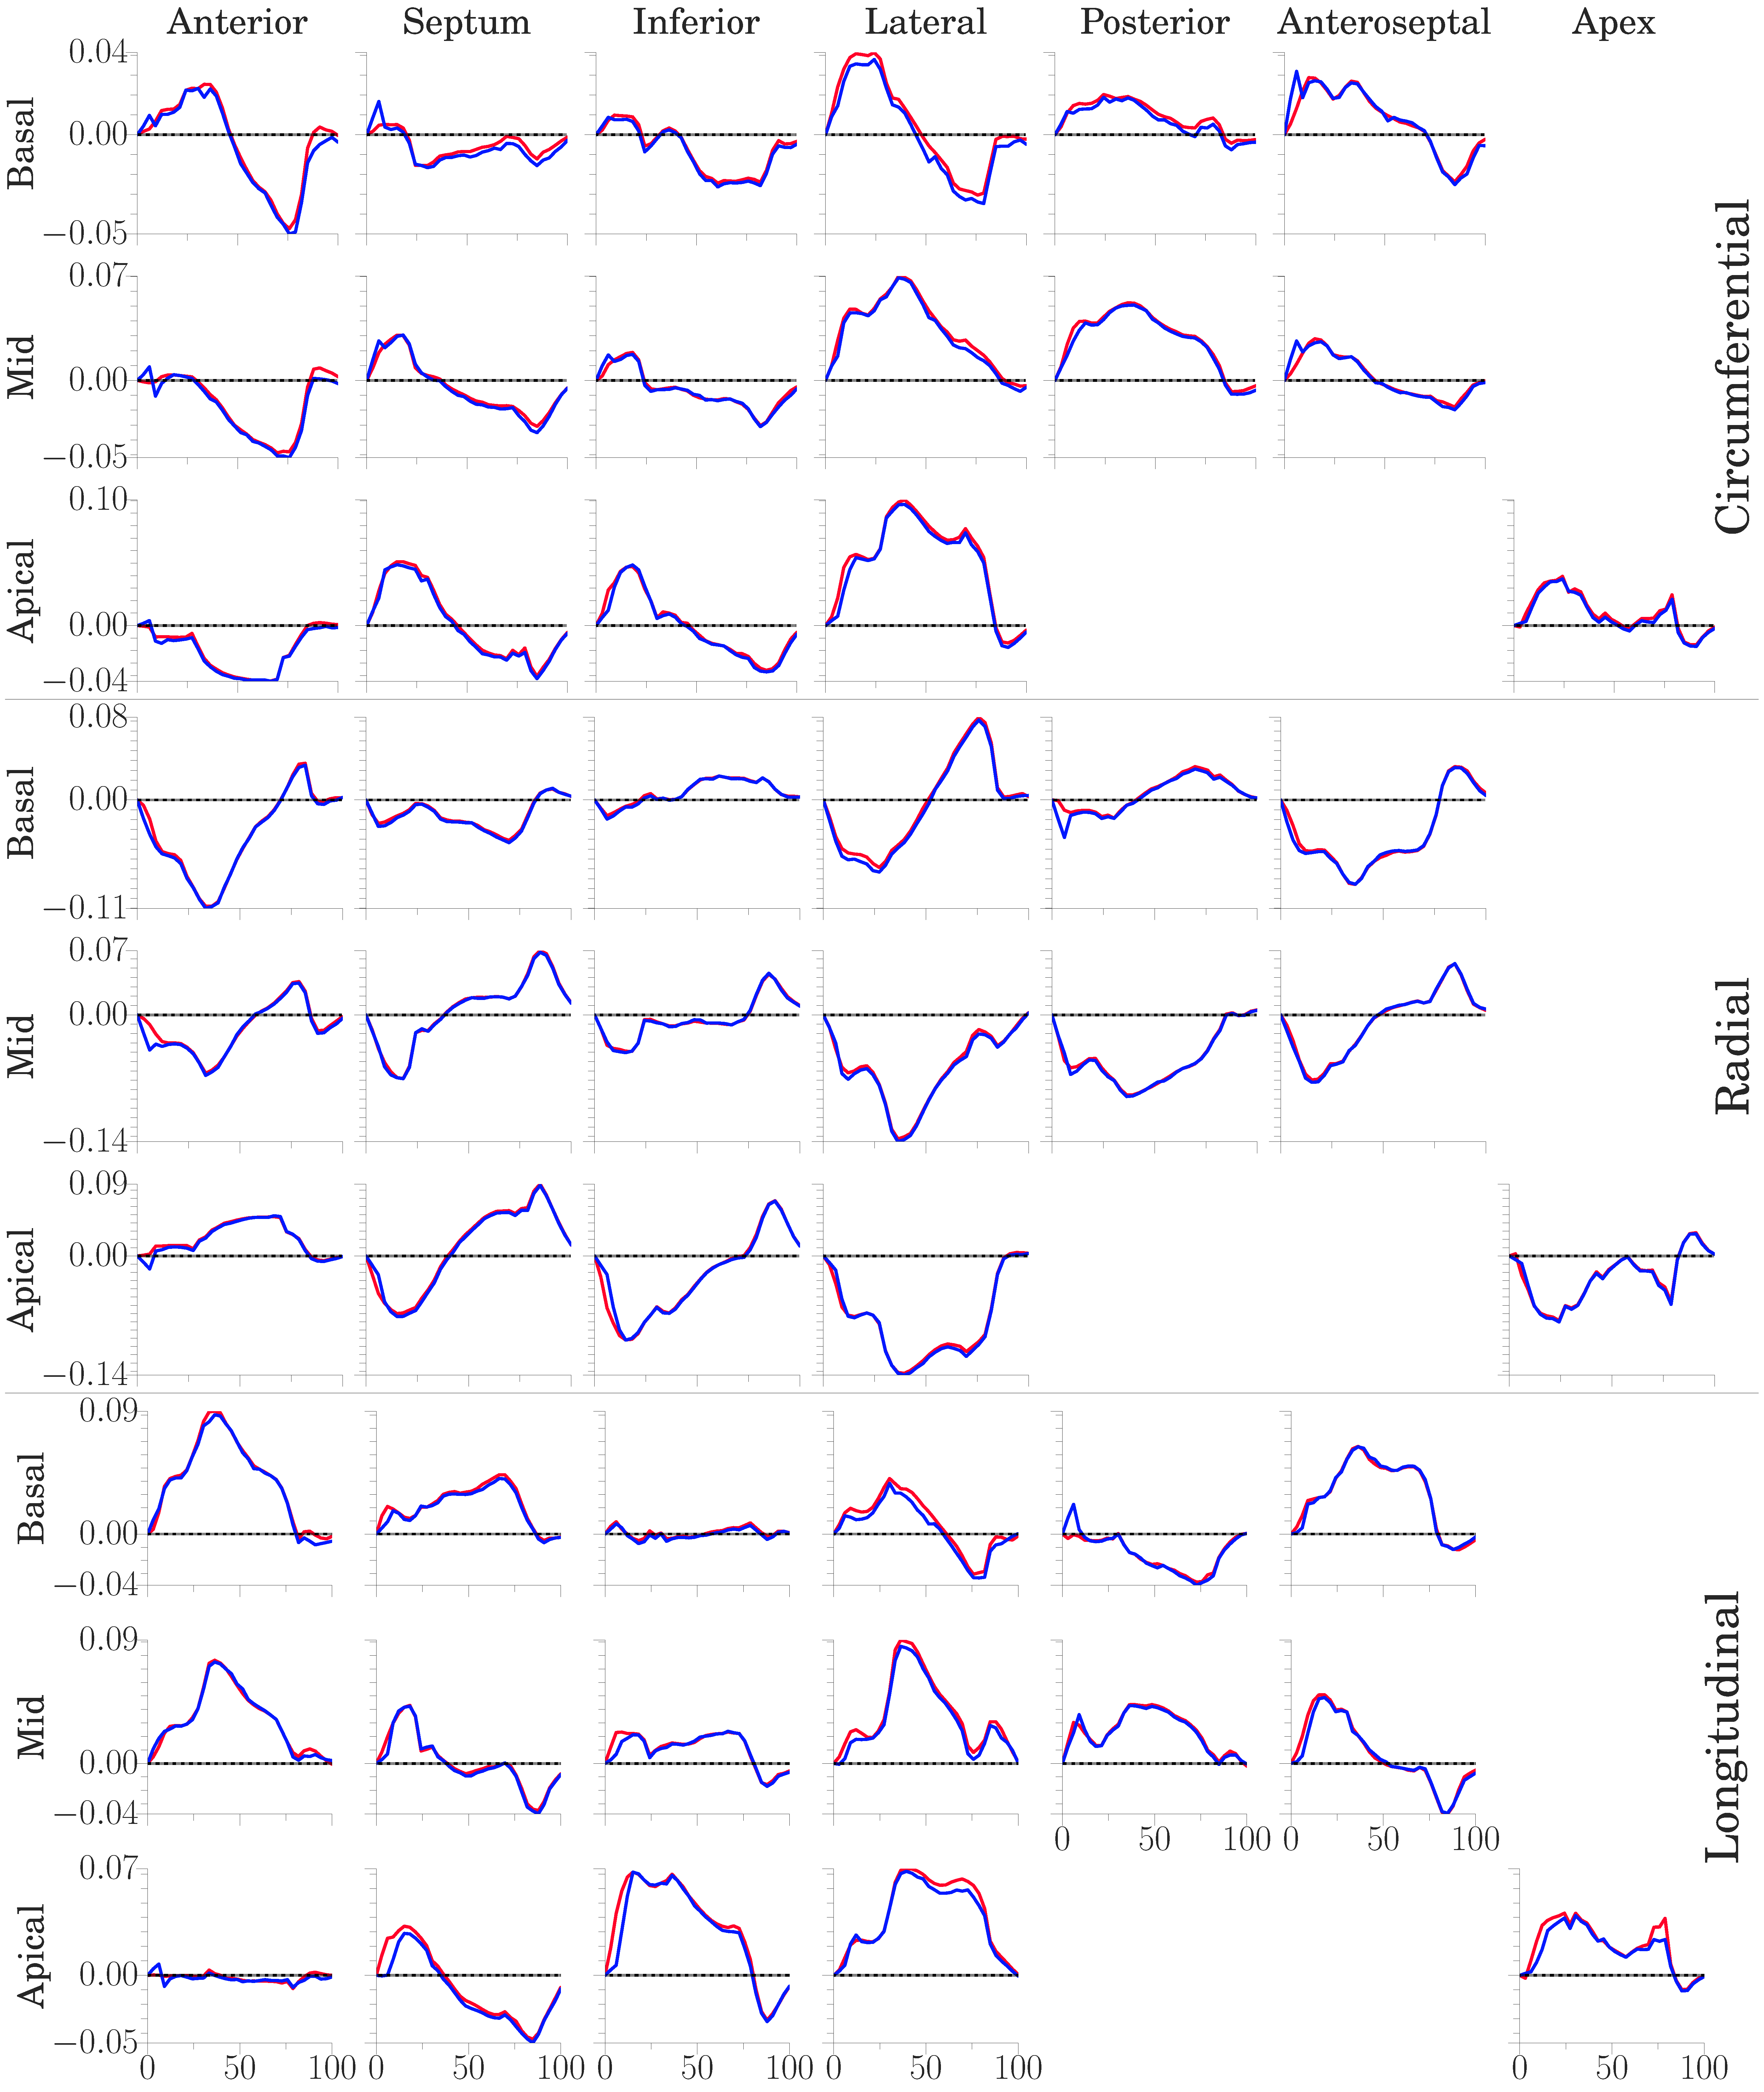
\includegraphics[width=\textwidth]{simulated_strains}
\caption{Comparison of regional strain curves starting in end diastole. In red: optimized wall
  motion model data. In blue: clinical data from speckle tracking
  echocardiography. In each plot the $y$-axis represents strain while
  the $x$-axis shows the progression in time of the cardiac cycle as a
  percentage.}
  \label{paper1:fig:strain_match}
\end{figure}

\begin{figure}[htbp]
\centering
    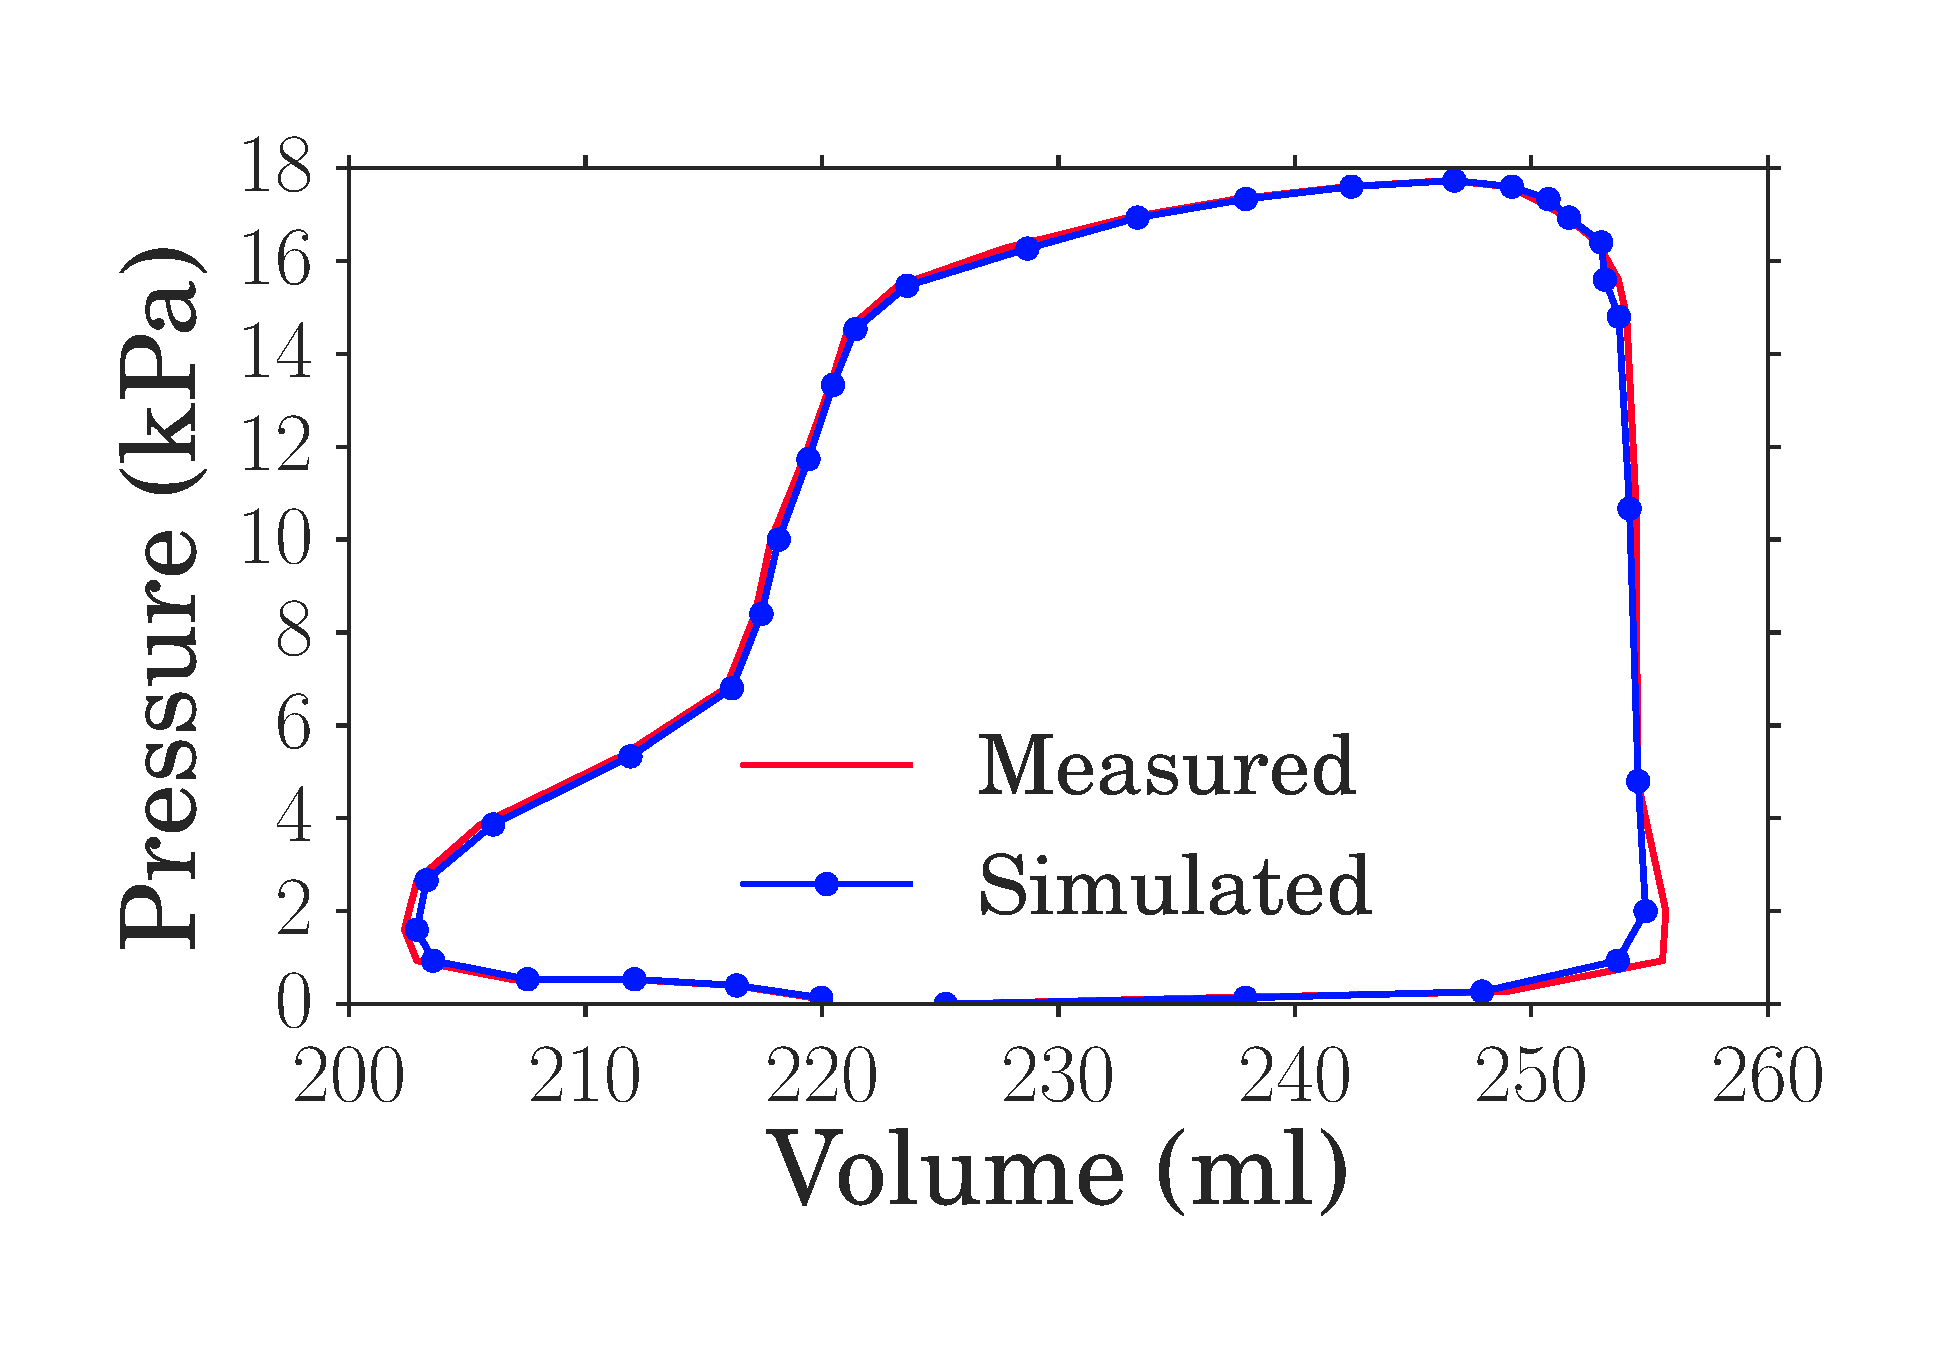
\includegraphics[width=0.7\textwidth]{simulated_pv_loop}
\caption{Clinically measured (red) versus optimized wall motion model
  (blue) left ventricular cavity volumes.}
\label{paper1:fig:pv_match}
\end{figure}

\begin{figure}[htbp]
\centering
    \includegraphics[width=\textwidth]{patient_gamma_snapshots}
\caption{Posterior view of the contraction field $\gamma$ optimized to in-vivo data 
at P1 resolution. A snapshot is shown for every third in-vivo measurement point.}
\label{paper1:fig:snap_shots}
\end{figure}


\subsection{Effect of contraction parameter resolution}
In order to quantify the effects of the resolution of the contraction field $\gamma$
we have repeated the contraction estimation from in-vivo data using regional and scalar resolutions.
The fit values obtained for these resolutions are compared to the fit value of the P1 resolution in Table~\ref{paper1:tab:gamma_space_opt_misfit}.
The results show that the P1 resolution of $\gamma$ gives an order of magnitude better strain and volume
matches than the scalar and regional resolutions, and that $\Istrainrelmax$
is about an order of magnitude lower than $\overline{I}_{\mathrm{strain}}$ in all three cases.

The computational cost of the data assimilation using the three resolutions of $\gamma$ is compared in 
Table~\ref{paper1:tab:patient_opt_details}. We note that the number of forward and adjoint solves 
increases with the resolution and that the average runtime of an adjoint solve in the scalar and P1 resolutions
are almost the same.

\begin{table}
  \centering
\caption{Performance of the contraction optimization with the clinical data for different
resolutions of contraction parameter $\gamma$.
The second and third column display the average number of forward and adjoint solves required to
optimize $\gamma$ at a single measurement point. The fourth column shows the total run time over all measurement points and
the final column the average run time of an adjoint solve. }
\begin{tabular}{lrrrr}
\hline
 resolution of $\gamma$ & forward solves &    adjoint solves &   total run time (s)  & adjoint evaluation \\
                       &  average        & average           &                       & average run time (s) \\
\hline
 scalar                &                   4.6  &                   2.8 &    280   & 7.4 \\ %(0.082) 
 regional              &                   12   &                   6.5 &    210   & 19.3 \\ %(0.062)
 P1                    &                   46   &                   46  &    1100  & 7.9 \\ %(0.11)
\hline
\end{tabular}
\label{paper1:tab:patient_opt_details}
\end{table}



\begin{table}
\caption{Relative misfit for different representation of $\gamma$}
\begin{tabular}{lrrr}
\hline
 resolution of $\gamma$ &   $\Ivolavg$ &   $\Istrainavg$  &    $\Istrainrelmax$ \\
\hline
 scalar           &                          0.044  &                                              1.5  &                                             0.27  \\
 regional         &                          0.024  &                                              1.1  &                                             0.16  \\
 P1               &                          0.0037 &                                              0.17 &                                             0.029 \\
\hline
\end{tabular}
\label{paper1:tab:gamma_space_opt_misfit}
\end{table}



\section{Discussion}
\label{paper1:sec:discussion}
In our study we have created a personalized model of whole cycle ventricular mechanics
based on strain, volume and pressure measurements of a dyssynchronous left ventricle. 
The contraction parameter in our study was resolved at a high P1 level of resolution.
Previous studies \cite{wong2015velocity, chabiniok2012estimation} have considered
contraction parameters that were resolved up to the regional level of AHA zones. By comparing
our P1 results to those generated with a regional resolution we have shown that it is possible
to greatly increase the fitting ability of a data assimilation method by increasing the 
parameter resolution. Indeed Table~\ref{paper1:tab:gamma_space_opt_misfit} shows 
that the fits $\Ivolavg$, $\Istrainavg$, and  $\Istrainrelmax$ are an order of magnitude better for
the P1 resolution as compared to the regional or scalar resolutions. 

Errors in strain fitting were significant at the P1 resolution when compared 
to the sizes of the strain curves ($\Istrainavg = 0.17$). These errors can 
stem from a fundamental model-data 
mismatch, and or an inability of the data assimilation to fit the model to the data. 
In the case of a model-data mismatch the limitations of the model may play a role (see Section \ref{paper1:sec:limitations}).
Another cause of model-data mismatch
is inaccuracy or noise in measurements, in which case the model can be used to improve 
the measurements. This is the case when models are used to regularize image based motion
\cite{papademetris2002estimation, tuyisenge2016estimation}. 

The SQP optimization algorithm that we employed is a local search only, so that is possible that
our fitting was suboptimal, possibly contributing to the mismatch in strain. Adding regularization
has been shown to prevent such suboptimal results in fluid control problems [\cite{gunzburger2003perspectives}~page 123].
This partially motivated our use of regularization in the contraction optimization \eqref{paper1:eq:opt_gamma}.

The discrepancies between our model based and measured strains are very small however when compared to
the sizes of the largest strain curves of a given strain type, longitudinal, 
circumferential or radial. This can clearly be seen in Figure~\ref{paper1:fig:strain_match}
and in the low value of the metric $\Istrainrelmax$. This shows that our method was able
to accurately capture the larger amplitude features of the heterogeneity in contraction. 
Such features are less prone to distortion by noise then those with smaller strain values, and are
therefore more relevant for potential medical use. However, the question of how much 
model resolution is actually needed to provide medically useful information 
remains an open one.

As a consequence of increased dimensionality in the optimization, 
estimating the contraction $\gamma$ took just under
4 times longer with the P1 resolution than the scalar resolution.
This was due to an increase in the number of 
forward and adjoint evaluations needed at the higher resolution. 
However the average run time of an adjoint gradient evaluation
did not differ significantly in the P1 case.  This near invariance 
of the gradient calculation cost to the number of optimization 
parameters is an advantage of the adjoint-gradient
method. In the case of the regional resolution the average adjoint-gradient 
run-time was nearly double that of the other two cases.
This was due to increased symbolic computation required by the 
software dolfin-adjoint to differentiate characteristic
functions defined over each AHA segment. The total run-time for the 
scalar case was higher than for the regional case, despite the
scalar case requiring fewer forward and adjoint evaluations. This was due to 
a greater number of Newton iterations 
required per forward solve in the scalar case.

In order to test the effects of mesh resolution on the contraction estimation we have considered
alternative mesh resolutions in Appendix~\ref{paper1:sec:mesh_res}. The analysis shows that 
the tested increase and decrease
in the resolution of the mesh did not significantly change the 
fit quality of the contraction estimation (Table \ref{paper1:tab:mesh_conv_opt_misfit}).
There were however slight differences in the spatial average of the contraction field 
between the three cases tested
(Figure \ref{paper1:fig:mesh_conv_gamma}). This was most likely due to differences 
in the quality of the discrete approximation of 
the work balance equation \eqref{paper1:eq:work-balance}.


In the current study the 
resolution of the computational mesh effected both the resolution of the contraction 
field and the resolution of the displacement-pressure variables	 in the FE model.
The results of the mesh resolution tests suggest our contraction field may have
been too highly resolved, and that it might be beneficial
to select the resolution of the contraction variable independently of the mesh
in future studies. This would require specifying a set of basis functions for $\gamma$, 
which could be designed to allow for a good fit of model to data while
at the same time minimizing the number of degrees of freedom.
Such a procedure has been previously implemented for parameter 
estimation in groundwater modelling \cite{tsai2003global}.

In order to test the accuracy of the contraction estimation 
we have conducted synthetic data tests for which the true
contraction field was known. The results of these tests
show that our data assimilation is greatly effected by the 
sparsity of data. Indeed the approximation of $\gamma$ was an order of magnitude better with strains
that had all 6 components and were defined everywhere on the geometry, 
as compared to the regionally averaged strains limited
to the tensor diagonal. This result did not hold at the apex where
the maximum errors were the same for all three cases.

The regionally averaged strain representation is easier for a
human to interpret and is widely used in 
medical research. However for the purposes of building accurate personalized models, 
more resolution of strain is highly advantageous.
The synthetic tests also showed that our data assimilation 
is not greatly effected by noise in the echocardiographic measurements. 
This is most likely due to our use of regularization, which favoured
smoother solutions that averaged out the effects of the noise. 

In addition to noise in strain we can also expect inaccuracies in volume measurements from echocardiography.
This is an issue for the estimation of the elastic parameter $a$, which we conducted purely from volume measurements.
Experiments with gel phantoms have quantified this inaccuracy for assessments of a single image \cite{aurich2014assessment}. 
However for the estimation of the elastic parameter $a$ relative differences in errors between images are more relevant.
These have to the best of our knowledge not been studied, and so we have conducted estimations of $a$ 
with volume curves perturbed by a range of errors (see Appendix \ref{paper1:sec:elasticparam}). 
These experiments show that the estimated stiffness parameter is indeed sensitive to volume errors. The effect on
the average of the contraction field is however quite minimal. 
An alternative to the current stiffness estimation procedure would be to allow
for greater spatial resolution from strain measurements as per the contraction parameter. 
This might allow for a regularized stiffness field to average out the effects of noisy measurements.

The volume fit between model and data was close for the three points in atrial systole, but significant
in early isovolumic contraction. Indeed the model underestimated the measured volumes,
indicating an overestimation of ventricular stiffness at these points. This is a consequence of 
fitting the stiffness parameters to the atrial systolic points, and not to the points afterwards. If the effects
of contraction could be isolated from the effects of elasticity it would be possible to 
include these points in the elastic parameter fitting and possibly obtain a better match of volumes.

In our study we personalized only a single elastic parameter $a$, which was done for the sake of simplicity.
Previous studies have successfully estimated greater numbers of elastic parameters for the reduced Holzapfel
law \cite{asner2015estimation} and the fully orthortropic Holzapfel law \cite{gao2015parameter}.
Such procedures could be potentially combined with our 
contraction estimation in order to increase the level of model personalization.
Another potential improvement of the elastic parameter estimation we employed 
is the inclusion of aggregated geometry measures;
such as short axis and long axis diameters. Such measures have been shown
to improve identifiability of elastic parameters in experiments
with mouse ventricles \cite{nordbo2014computational}.


Several data assimilation studies \cite{mojsejenko2014estimating,
  sun2009computationally} have included objective functionals
consisting of strain and volume components with equal weighing given
to both. We have shown that it may be possible to improve such data
assimilation procedures by tuning the relative weight of strain and
volume components. Indeed in the top right plot of Figure~\ref{paper1:fig:lcurves} there is 
a definite corner in the strain-volume fitting space consisting of 4 points
beneath $\alpha = 0.95$. Choosing $\alpha$ among these points gives
a fair trade-off between strain and volume matching whereas any choice outside this
corner simply worsens the fit of strain or volume without much improving the other.

In Figure~\ref{paper1:fig:lcurves} we have shown how the parameters $\alpha$
and $\lambda$ effect the fitting and smoothness 
 metrics related to the contraction field $\gamma$. Additionally, we have
tested the effects of variations in $\alpha$ and $\lambda$ on the spatial
average of the contraction field. These experiments are presented in Appendix~\ref{paper1:sec:sense_alpha_lambda}.
Figure~\ref{paper1:fig:gamma_sense_alpha_lambda} shows that varying $\alpha$ in the region $[0, 0.5]$ had little to no effect on the spatial average of
$\gamma$, whereas increases in $\alpha$ outside of this region tended to increase the amount of 
contraction. This behaviour correlates with the value of $\Istrainavg$ in (Figure~\ref{paper1:fig:lcurves}
top right). Similarly, increasing $\lambda$ beyond $0.001$ tended to increase the misfit in the data 
functional (Figure~\ref{paper1:fig:lcurves} bottom right), and also increase the average amount of
contraction (Figure~\ref{paper1:fig:gamma_sense_alpha_lambda} right).
We hypothesize that additional levels of misfit in strain introduced by increasing
$\alpha$ beyond $0.5$ and or $\lambda$ beyond $0.001$ lead to overestimating 
the amount of contraction in our patient's LV. However we lack knowledge of the
true amount of muscle contraction in the patient which could be used to test the hypothesis.
Further validation of the model and data assimilation are needed.


\subsection{Limitations}
\label{paper1:sec:limitations}
The results obtained in this article were limited by issues pertaining
to the choice of mathematical model, quality of clinical data,
numerical stability, and the design of the data assimilation
algorithm.  Firstly, the boundary conditions of the ventricle wall
motion model did not account for the effects of the right ventricular
pressure on the septum, and the mechanical coupling to the
neighboring structures: left atrium, right ventricle and pericardium.

The in-vivo circumferential and radial motion at the base was not incorporated into the model.
Instead some motion was allowed by the basal spring, whose constant $k$ needed to be chosen.
In the future we would like to
incorporate basal motion data from the images into our personalized model. This would
allow us to avoid having to make a choice of $k$ and hopefully allow for the
reproduction of in-vivo basal motion in the personalized model.

During the atrial systole phase we assumed $\gamma = 0$. This allowed for 
the estimation of passive properties separate from contraction. This assumption 
is appropriate for a healthy ventricle but
might be false in a diseased ventricle if muscle relaxation is sufficiently delayed.

Our mathematical model of wall motion neglected the effects of
visco-elasticity, tissue compressibility \cite{yin1996compressibility},
inertia, and myocardial sheet
microstructure. Finally the reference geometry that we used for our
calculations came from an echocardiographic image in which there was a
non-zero level of blood pressure.  The blood pressures we used in our
patient specific model were off by the 2.8 kPa which we subtracted in
order to have 0 pressure in the reference geometry.  This pressure
adjustment meant that the elastic stiffness of the ventricle was
underestimated by our elastic parameter estimation, as the
mathematical model operated at a lower pressure than measured in the
patient's heart.

The accuracy of the optimized motion model is limited by uncertainties
in the clinical strain and volume measurements,
which are related to echocardiographic image quality,
image sample rate, and speckle tracking algorithm accuracy. 
Pressure and volume measurements had to be synchronized, which might
have lead to a potentially unphysiological loss of volume in the iso-volumic relaxation phase of
the in-vivo PV loop (Figure~\ref{paper1:fig:pv_loop_phases}).

Finally there were several algorithmic limitations. 
Firstly, the optimized $\gamma$ fields we computed may or may not have been unique.
For potential clinical applications this is a concern as the uniqueness of parameters
relate to the reproducibility and consistency of data obtained from a personalized
model. Furthermore, our procedures for
choosing the functional weights $\alpha$ and $\lambda$ were not optimal.
In both the synthetic
and clinical data case the weight values
were chosen by parameter sweeps that kept a single parameter fixed, which did not
account for possibly better $\alpha,\lambda$ combinations
lying outside of the areas we tested. 
Finally the SQP optimization algorithm that we employed 
was a local search only, that is only
one minimum of the objective is calculated. Better parameter fits may be possible
with global optimization methods that explore multiple minima.

\section{Conclusion and Future Outlook}
\label{paper1:sec:conclusion}
By employing high resolution data assimilation we
were able to capture the detailed motion of a dyssynchronous left
ventricle in a computational model with an excellent fit of model observations
to data. This demonstrates the power of the data assimilation method,
which can also be applied to other models and or model parameters.

In the future the proposed method should be further improved and 
tested on cohorts of patients. This would allow for the study of simulated contraction patterns 
among groups of patients that could lead to further understanding of
dyssynchrony.

\section{Author Declaration}
All of the clinical data for this study was collected with the approval of the Norwegian national ethics committee, REC,
and in accordance to the Helsinki Declaration of 1975, as revised in 2000.

% \ack
Computations were performed on the Abel supercomputing cluster at the
University of Oslo via Notur projects nn9316k and nn9249k.

\section{Appendix}

\subsection{Sensitivity of elastic $a$ parameter to error in atrial systolic volume measurements}
In order to test the sensitivity of our estimated $a$ parameter to
uncertainty in volume measurements we have carried out a series of estimations with
various levels of volume perturbation. 
We generated clean volume data using the computational model using $a = 0.435$ kPa, 
the optimal value obtained from the clinical data. Perturbations in volume increases
of sizes $\pm 5,15, 25 \%$ were added to this data,
which were then used as target for optimization. The resulting $a$ values and perturbations
are shown in Table~\ref{paper1:tab:passive_synth_opt}. The largest perturbations resulted
in the $a$ values 0.494 kPa and 0.384 kPa, representing circa $\pm \%13$ change from the original $a$ value.


\begin{table}
\caption{Sensitivity of the optimized material parameter $a$ to errors in volume measurements.
The first column gives the perturbation of the volume increase 
between measurement points 1-2 and 2-3, in percent. 
The next two columns give the size of these perturbations in mL with $\Delta V_2$ 
and $\Delta V_3$ referring to perturbations in the 
volumes of the second and third measurement points respectively. In the fourth column 
optimal $a$ values are given. In all cases 
the volume fit $\overline{I}_{\mathrm{vol}}$ was less than $4 \times 10^{-6}$.}
\begin{tabular}{rrrrr}
\hline
	 perturbation  &   $\Delta V_2$ &   $\Delta V_3$ &      $a$ \\
                ($\%$) &   (ml) &   (ml) &      (kPa) \\
\hline
                   -25 &              -1.2   &              -1.06  &    0.494 \\
%                   -20 &              -0.956 &              -0.848 &   0.481 \\
                   -15 &              -0.717 &              -0.636 &    0.469 \\
%                   -10 &              -0.478 &              -0.424 &   0.458 \\
                    -5 &              -0.239 &              -0.212 &    0.446 \\
                     0 &               0     &               0     &    0.435 \\
                     5 &               0.239 &               0.212 &    0.424 \\
%                    10 &               0.478 &               0.424 &   0.414 \\
                    15 &               0.717 &               0.636 &    0.404 \\
%                    20 &               0.956 &               0.848 &   0.394 \\
                    25 &               1.2   &               1.06  &    0.384 \\
\hline
\end{tabular}
\label{paper1:tab:passive_synth_opt}
\end{table}

The resulting average value of $\gamma$ is shown in
Figure~\ref{paper1:fig:gamma_sense_mat} for the extreme cases
with $\alpha = 0.494$ and $\alpha = 0.384$ . For reference we also include the
average value of $\gamma$ using $\alpha = 0.435$.
 
\begin{figure}[t]
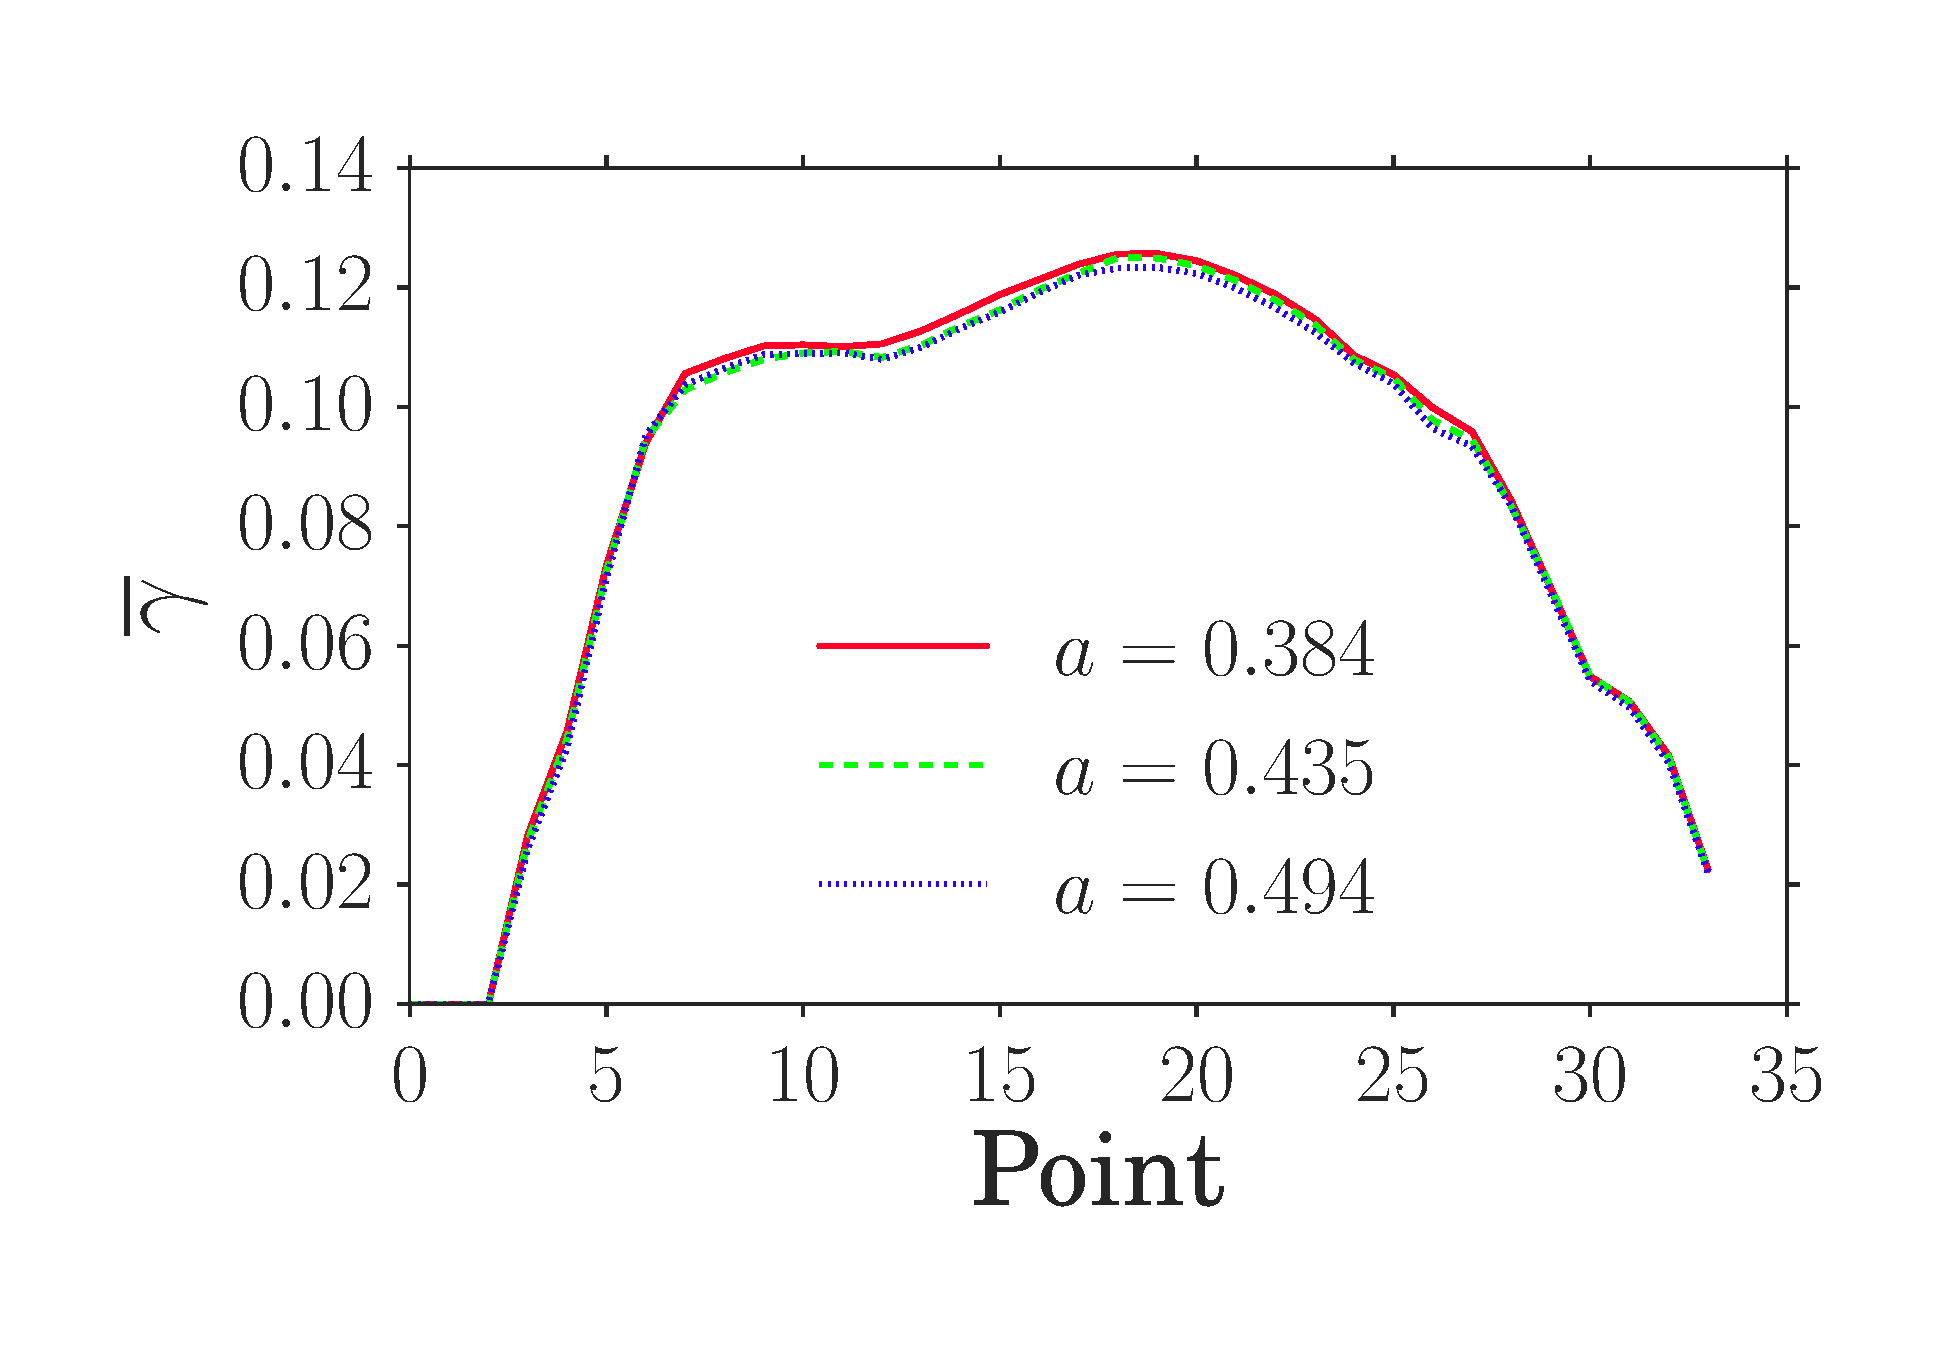
\includegraphics[width=0.7\textwidth]{mean_gamma_material_parameters_fixed}
\caption{Sensitivity of the optimal average contraction $\overline{\gamma}$ to changes in the parameter $a$. The upper and lower $a$
values are based on estimating $a$ with volume perturbations of $\pm 25 \% $ (Tabel~\ref{paper1:tab:passive_synth_opt}). The middle
 value was obtained by estimating $a$ from in-vivo volumes.}
\label{paper1:fig:gamma_sense_mat}
\end{figure}


\subsection{Sensitivity of estimated parameters to spring constant $k$.}
\label{paper1:sec:k_sense}
The spring boundary condition that we used at the ventricular base has a significant
effect on the simulated cavity volumes calculated by the model. This is due to the 
cross-sectional area of the cavity being large at the ventricular base. Therefore 
we can expect the choice of $k$ to have an effect on the optimal parameters calculated 
by our data assimilation. 

In order to quantify this effect we have
carried out a sensitivity analysis, starting with the effect of $k$ on the optimized elastic parameter $a$.
We repeated the elastic parameter fitting decribed in Section~\ref{paper1:sec:elasticparam} and varied the $k$-value from 0.001 to 100.0.
We also considered the case $k = \infty$, denoting a completely rigid boundary held by
Dirichlet boundary conditions. The effect of the choice of $k$ on the
optimal value of $a$ is shown in Table~\ref{paper1:tab:elast_sense}. The
table shows that the optimal $a$ varies from 0.365 kPa to 0.875 kPa depending upon how the $k$ parameter is set. 

We also tested the sensitivity of the contraction $\gamma$ at P1 resolution to $k$ by
repeating the estimation of $\gamma$ with the various $k$ and $a$ pairs obtained in the
previous experiment. For each $k, a$ pair we have plotted the spatial average of contraction $\overline{\gamma}$
at each measurement point in Figure~\ref{paper1:fig:gamma_sense}. The results
show up to a $20 \%$ variation in $\overline{\gamma}$ and
very little variation for the choices of $k$ greater than or equal to
1.0. For some of the values of $k < 1.0$ our homotopy Newton solver was unable to 
secure convergence during the optimization. Curves corresponding to
these cases are drawn only to the point before the non-convergence occurred.


\begin{table}
\caption{Sensitivity of optimal $a$ value to choice of spring constant
  $k$.}
\scalebox{0.8}{
\begin{tabular}{|l|llllllllllll|}
\hline
      $k$ & $10^{-8}$ & $10^{-7}$& $10^{-6}$&  $10^{-5}$  & $10^{-4}$ & $10^{-3}$ & 0.01 & 0.1 & 1 & 10 & 100 & $\infty$ \\
\hline
      $a$ & 0.875   & 0.875  & 0.875  & 0.875 & 0.873& 0.873 & 0.849 & 0.684 & 0.435 & 0.375& 0.366 & 0.365 \\
\hline
\end{tabular}}
\label{paper1:tab:elast_sense}
\end{table}

\begin{figure}[t]
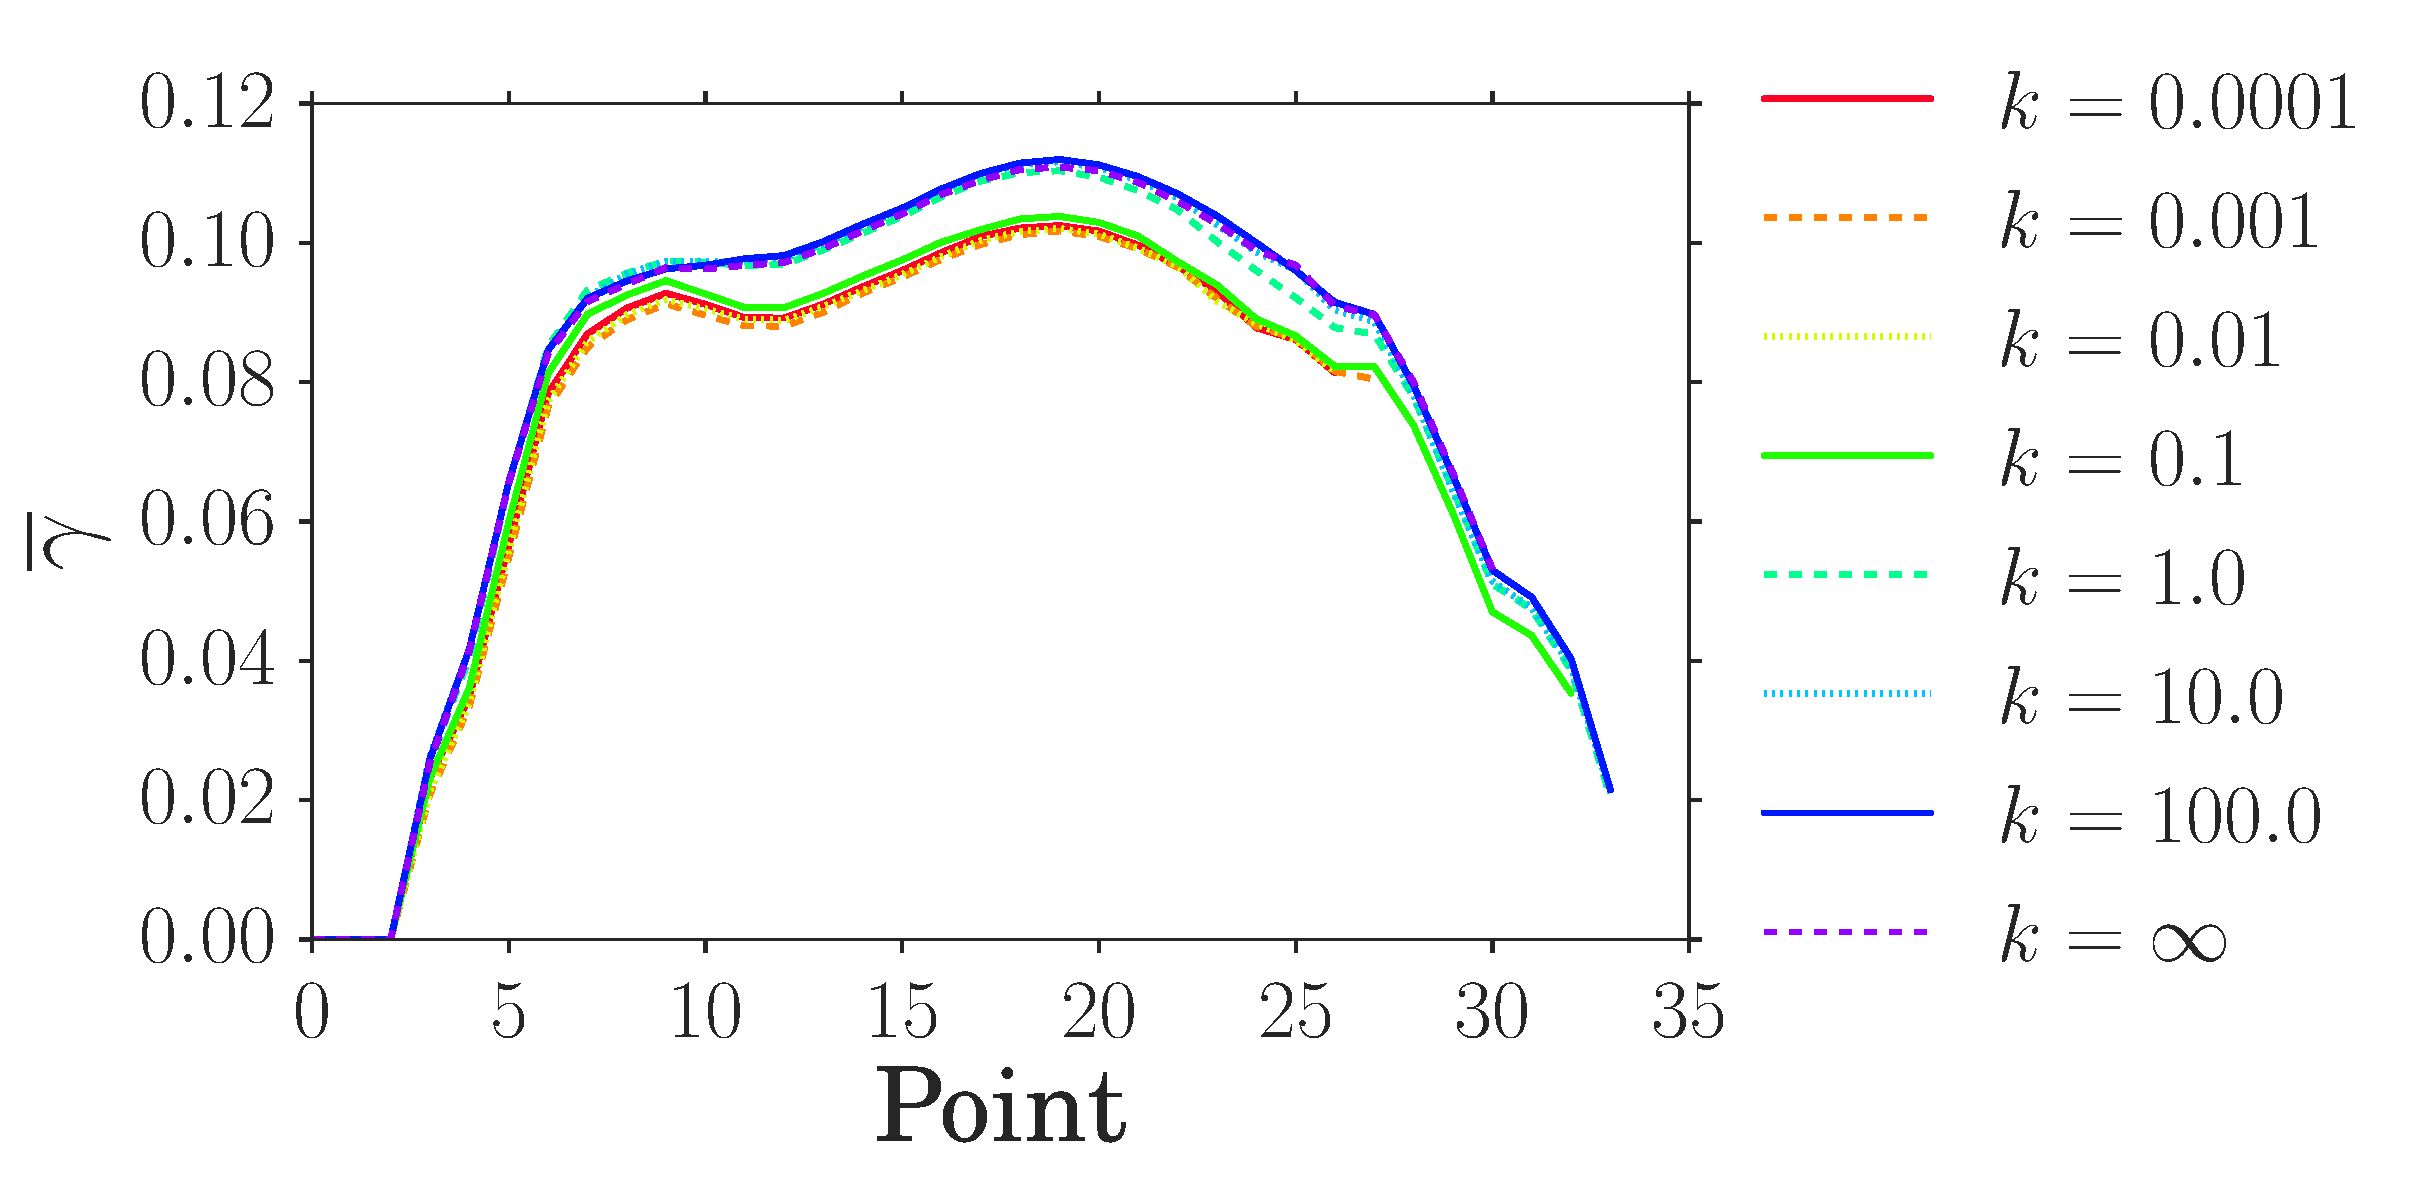
\includegraphics[width=0.7\textwidth]{gamma_mean}
\caption{Sensitivity of the spatially averaged 
contraction $\overline{\gamma}$ to the choice of spring constant $k$.}
\label{paper1:fig:gamma_sense}
\end{figure}


\subsection{Effect of mesh resolution on estimated contraction
  $\gamma$ at P1 resolution} 
\label{paper1:sec:mesh_res}
Ventricular meshes were generated by Gmsh
\cite{geuzaine2009gmsh} with three different resolutions controlled by the parameter
'Mesh.CharacteristicLengthFactor'.  This parameter
was given the values $1.0$, $0.65$ and $0.45$ which resulted in meshes with
$549$, $1262$ and $2261$ vertices respectively. Using the three meshes
we estimated contraction fields from the in-vivo data. The average value of
$\gamma$ is shown for these three cases in Figure~\ref{paper1:fig:mesh_conv_gamma}. 
Fit quality is compared in Table~\ref{paper1:tab:mesh_conv_opt_misfit}.

\begin{table}
\caption{Relative misfit for different mesh resolutions}
\begin{tabular}{llll}
\toprule
Number of elements & $\Ivolavg$ & $\Istrainavg$ & $\Istrainrelmax$ \\ 
\midrule
549  & 0.0033 & 0.17 & 0.029 \\
1262 & 0.0037 & 0.17 & 0.029 \\
2661 & 0.0043 & 0.18 & 0.031 \\
\bottomrule	
\end{tabular}
\label{paper1:tab:mesh_conv_opt_misfit}
\end{table}

\begin{figure}[]
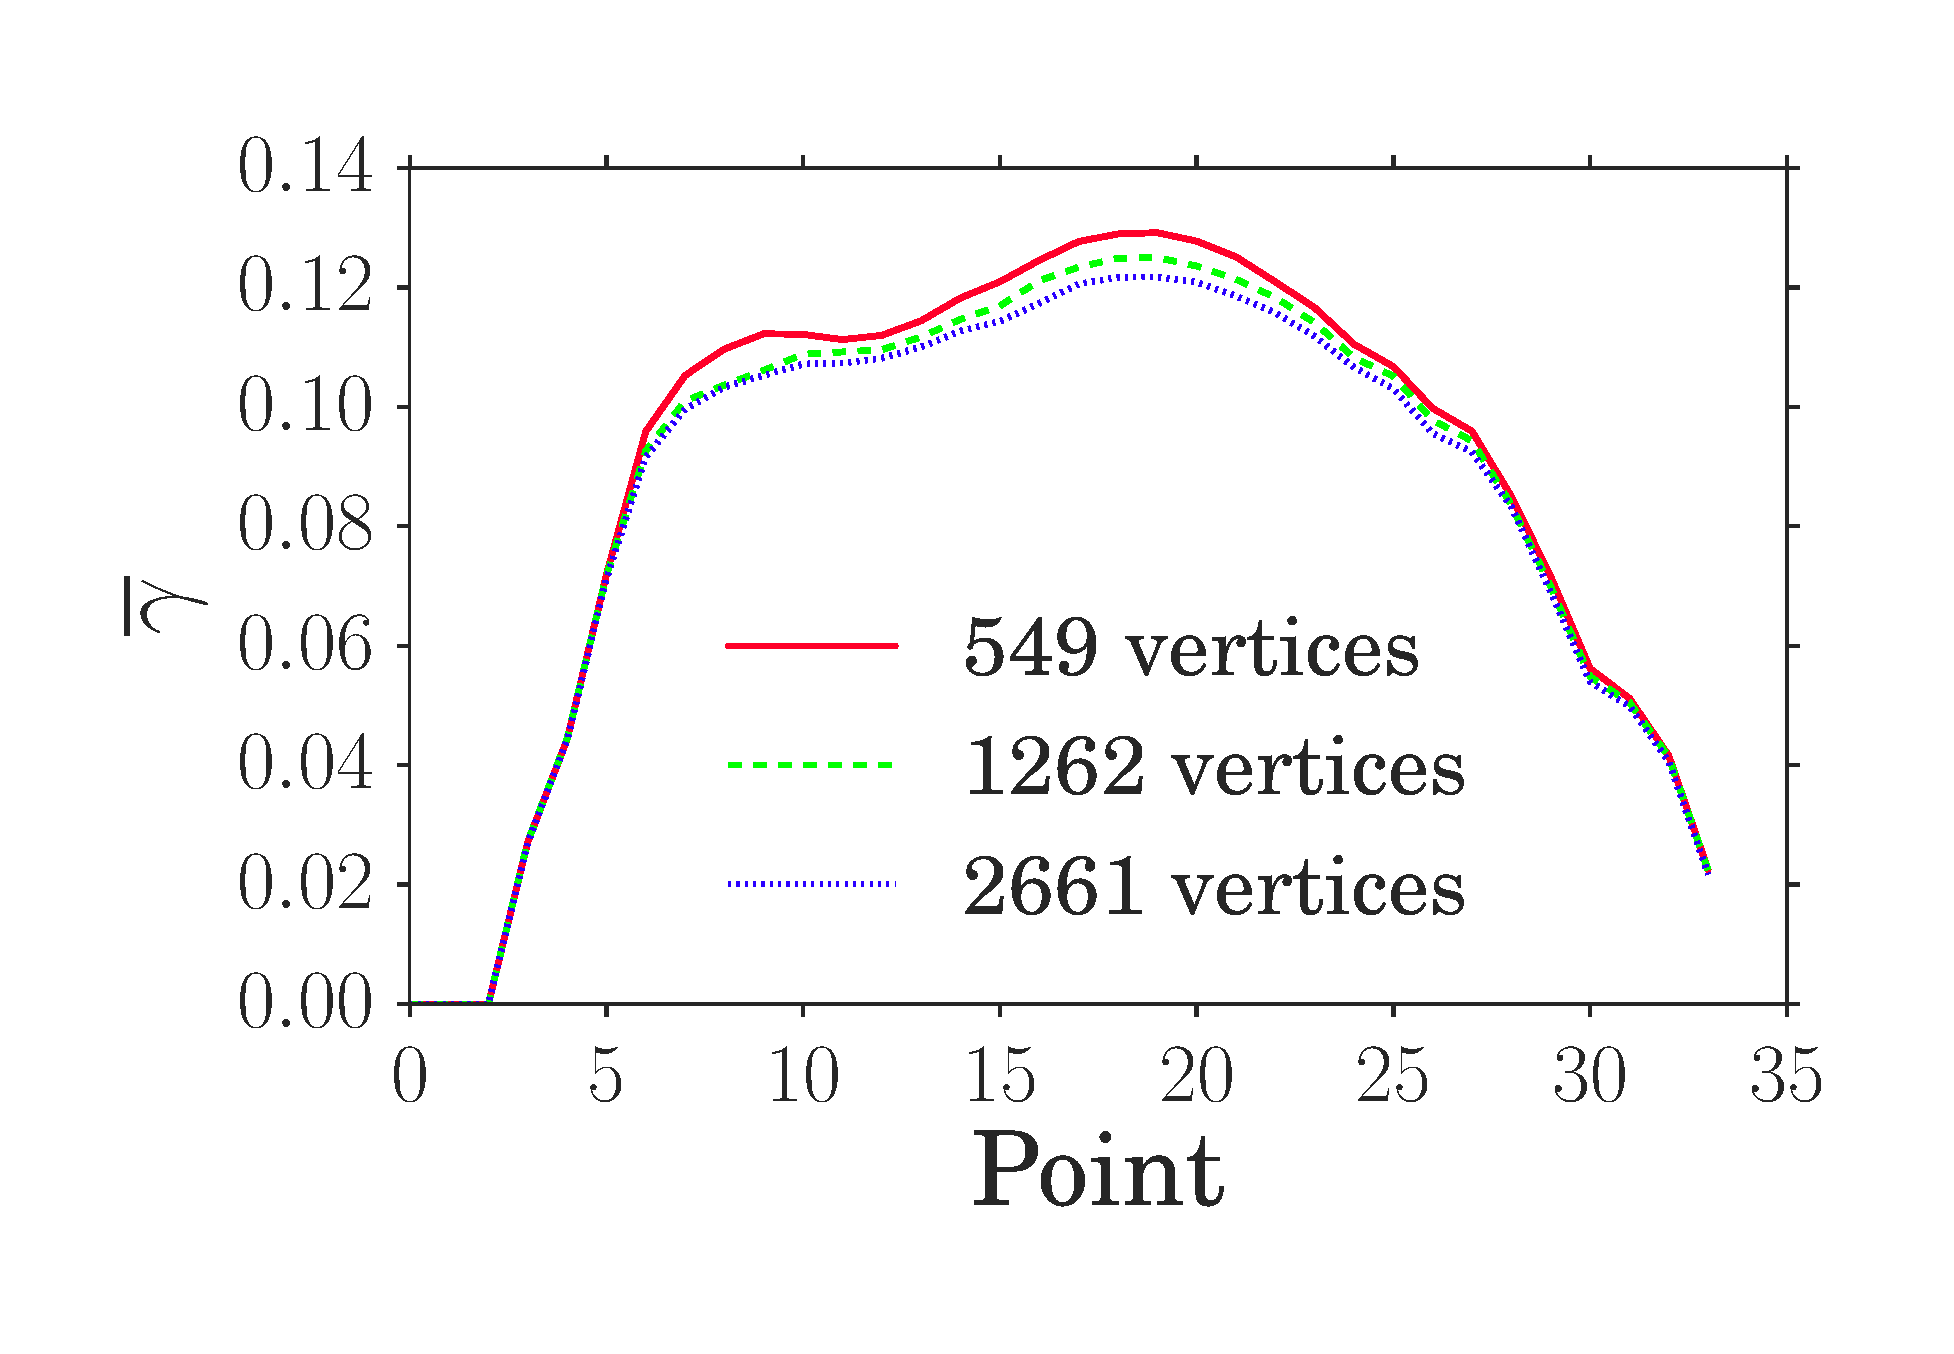
\includegraphics[width=0.6\textwidth]{mesh_conv_gamma}
\caption{Spatial average of contraction $\overline{\gamma}$ for 3 different mesh
  resolutions.}
\label{paper1:fig:mesh_conv_gamma}
\end{figure}


\subsection{Sensitivity of Contraction Size to choices of $\alpha$ and $\lambda$}
\label{paper1:sec:sense_alpha_lambda}
Based on the trade-off curves in Figure~\ref{paper1:fig:lcurves} we chose 
the optimization weights $\alpha = 0.95$ and $\lambda = 0.01$ for the personalization
of our wall motion model to the in-vivo data. In order to show the effect of these 
choices on the optimized contraction field $\gamma$ we have varied
the $\alpha$ and $\lambda$ values and plotted the spatial averages of the resulting
contraction fields. The results show that the amount of contraction tends to increase
proportionally to both $\alpha$ and $\lambda$ beyond the thresholds $\alpha = 0.5$ and
$\lambda = 0.001$. 

\begin{figure}[htbp]
\centering
\begin{subfigure}[t]{0.49\textwidth}
     {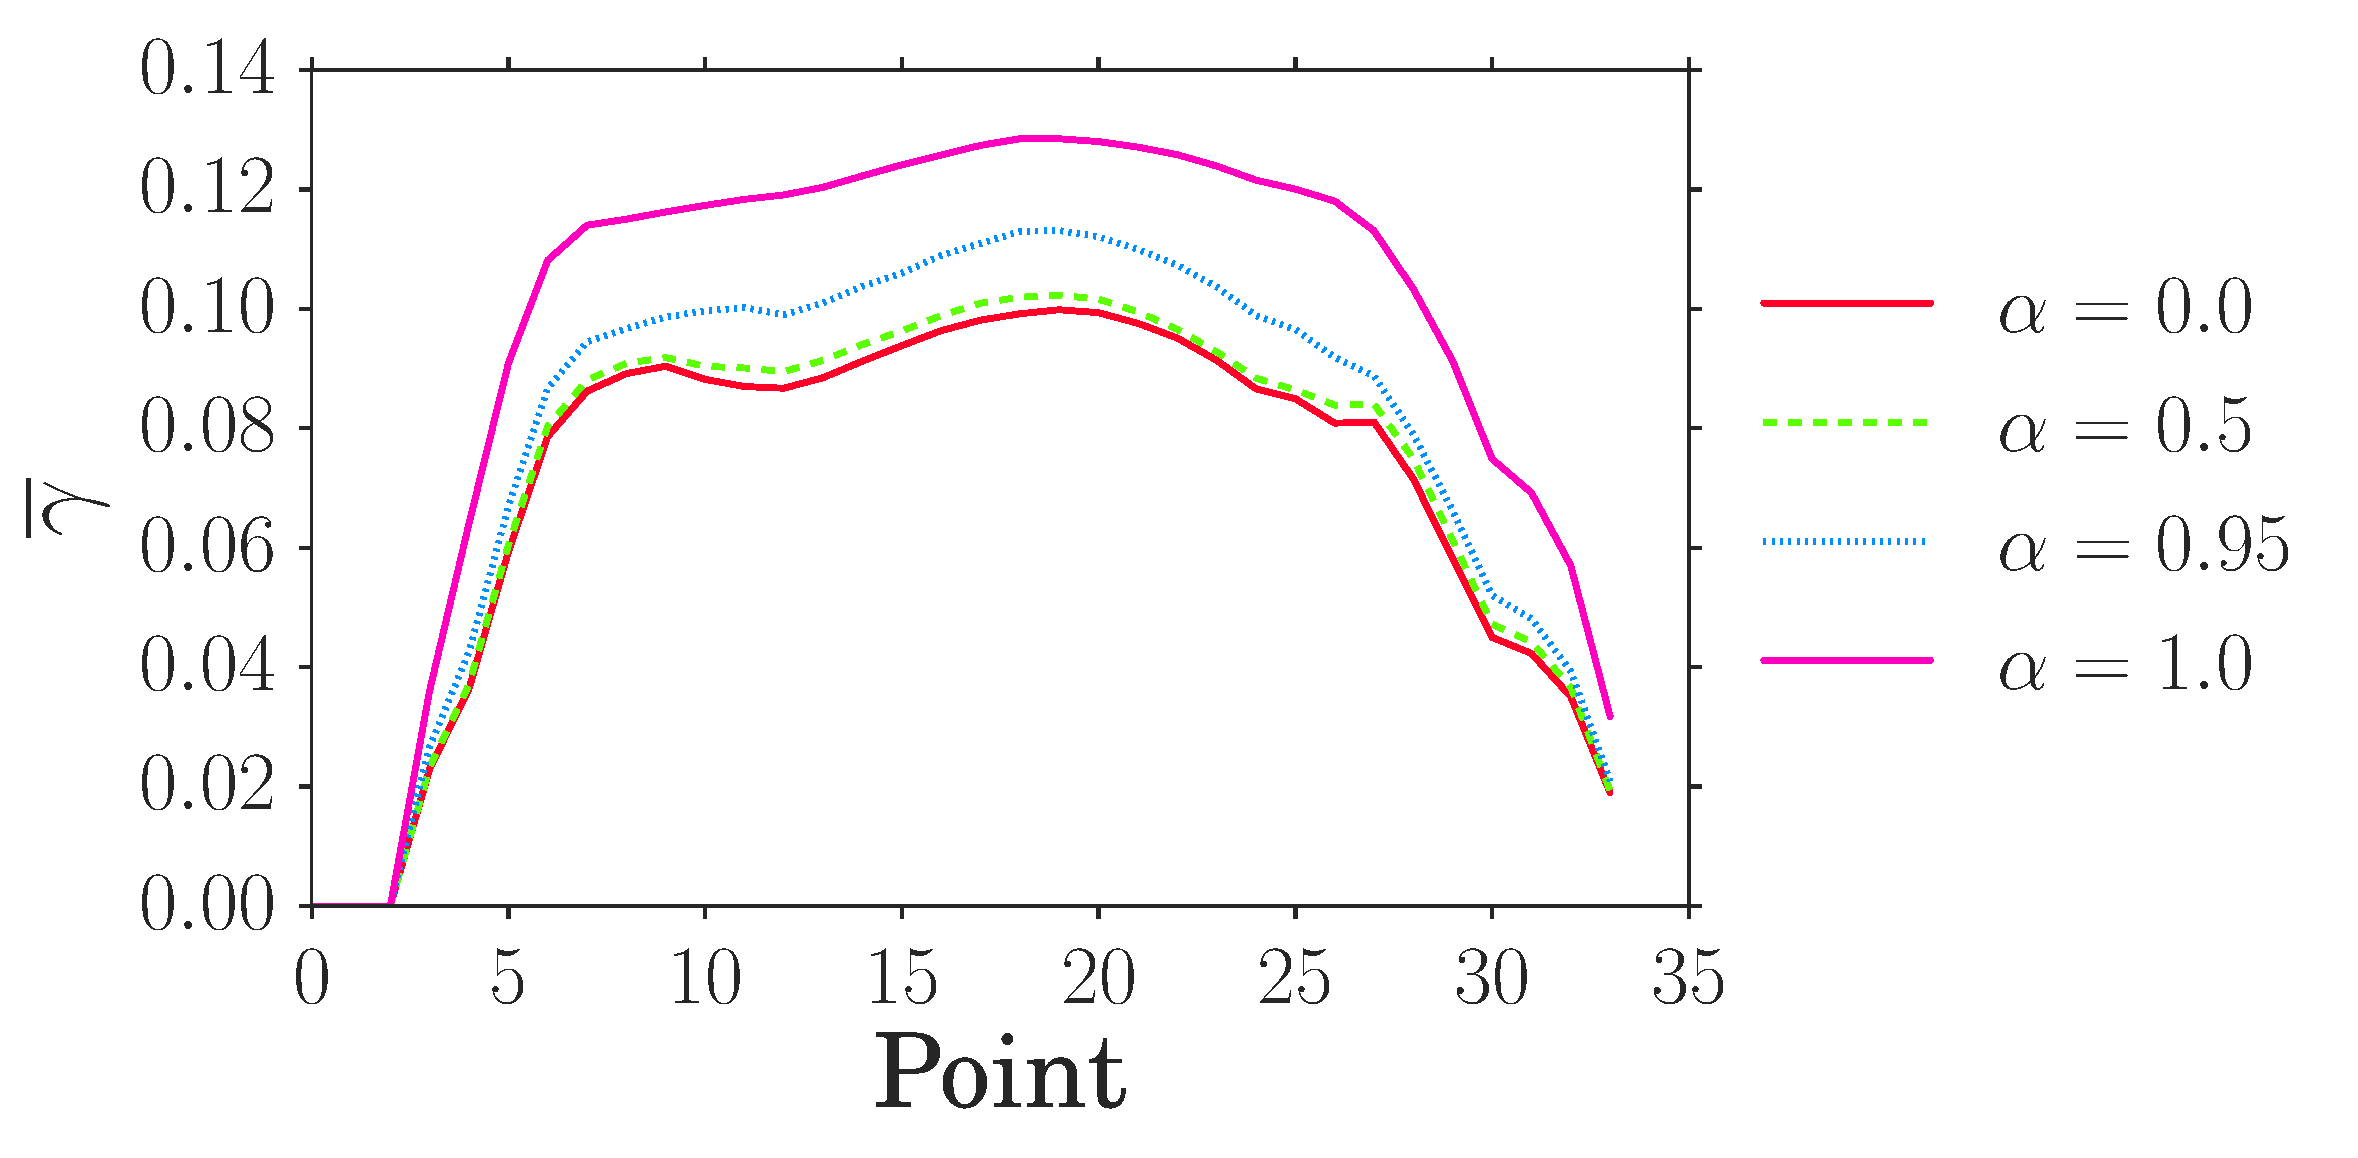
\includegraphics[width=\textwidth]{mean_gamma_varying_alpha}}
     \caption*{\label{paper1:fig:gamma_sense_alpha}}
\end{subfigure}
\begin{subfigure}[t]{0.49\textwidth}
    {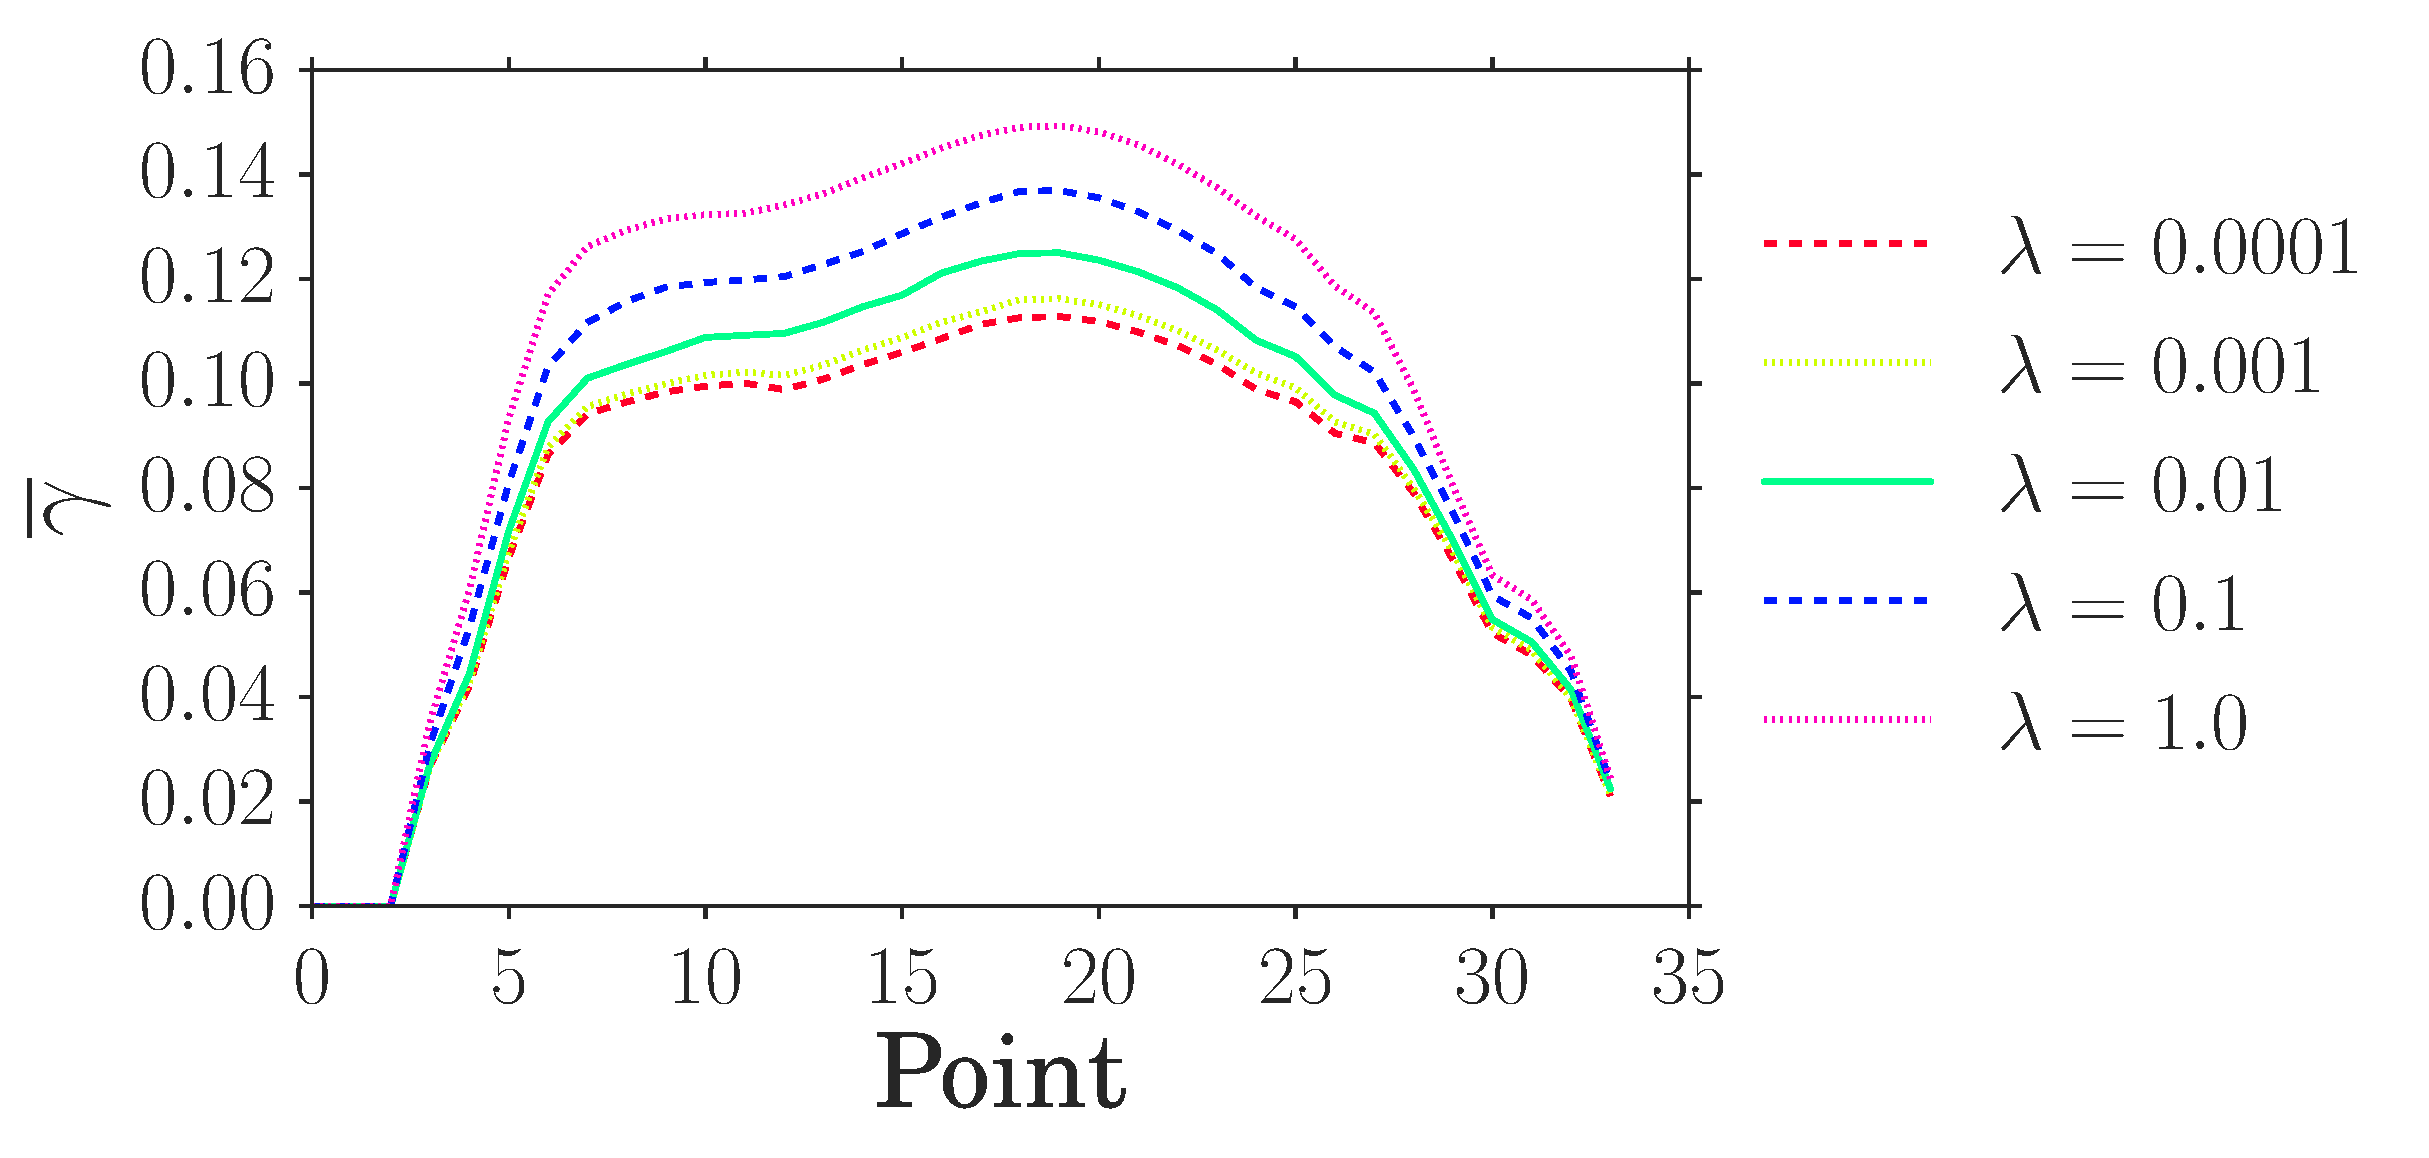
\includegraphics[width=\textwidth]{mean_gamma_varying_lambda}}
    \caption*{\label{paper1:fig:gamma_sense_lmbda}}
\end{subfigure}
\caption{Sensitivity of the spatially averaged contraction $\overline{\gamma}$ 
to variations in optimization weights $\alpha$ and $\lambda$. Left: $\lambda = 0$ and 
$\alpha$ is varied. Right: $\alpha = 0.95$ and $\lambda$ is varied.}
\label{paper1:fig:gamma_sense_alpha_lambda}
\end{figure}


\subsection{Estimation of noise in echo speckle tracking strain measurements}
\label{paper1:sec:strain_noise_est}
In order to increase the relevance of the synthetic tests we
considered a set of regional strains that contained noise. This
noise was modelled as an additive Gaussian process in order to imitate
the accumulation of tracking errors in EchoPac's image based strain
calculations. The mean and variance of a summand in the Gaussian
process were estimated from our in-vivo strain data of a single patient. From this data 
the sample means and variances of
the drift values were divided by the number of measurement points in order to approximate the noise in 
a single measurement. The mean and covariance of this single measurement point noise are given in
Table~\ref{paper1:tab:noise_covar_mean}.Theoretically, error free strain
curves would have no drift given stable conditions in the heart.
This motivates the use of the drift values in order to approximate 
the tracking error.

\begin{table}
  \caption{Mean and covariance of a Gaussian noise summand
    estimated from patient drift values in circumferential (C), radial
    (R) and longitudinal (L) directions.}
  \begin{center}
    \begin{tabular}{|l|ccc|c|}
      \hline
      & \multicolumn{3}{l|}{Covariance $\times 10^{-4}$} & Mean \\
      & C & R & L & \\
      \hline
      C &1.43 & 0.73 & 0.66  & 0.006 \\
      R& -    & 6.8 & 6.31  & -0.013 \\
      L &  -   &  -   & 7.26 & 0.01  \\
      \hline
    \end{tabular}
    \label{paper1:tab:noise_covar_mean}
  \end{center}
\end{table}




% \FloatBarrier
% \pagebreak
\newpage
\bibliographystyle{plain}
\bibliography{chapters/paper1/bibliography}

% \end{document}


%%% Local Variables:
%%% mode: latex
%%% TeX-master: "../../main"
%%% End:
